% TRANSFORMATIONAL AUTONOMOUS ENTERPRISES — Writer #4 research edition.
% Complete single-file source: all sections, vector figure bodies and bibliography embedded.
% Compile twice with pdflatex (TeX Live 2023 or compatible packages).
% No shell escape, external assets, network access or BibTeX step is required for this file.
% Canonical editable modules, references.bib and vector SVG/PDF forms remain in the source archive.
\documentclass[11pt]{article}

% BEGIN style.tex
\usepackage[letterpaper,margin=0.78in,headheight=15pt,headsep=20pt,footskip=30pt]{geometry}
\usepackage[T1]{fontenc}
\usepackage[utf8]{inputenc}
\usepackage{lmodern,microtype,amsmath,amssymb,amsthm,graphicx,booktabs,tabularx,longtable,array}
\usepackage{pgfplots}
\pgfplotsset{compat=1.18}
\usepackage{enumitem,xcolor,tikz,tcolorbox,fancyhdr,titlesec,caption,csquotes,placeins}
\usepackage[numbers,sort&compress]{natbib}
\usepackage{xurl}
\usepackage[colorlinks=true,linkcolor=DeepPurple,citecolor=DeepPurple,urlcolor=DeepPurple,breaklinks=true]{hyperref}
\usetikzlibrary{arrows.meta,positioning,calc,fit,backgrounds}
\definecolor{DeepPurple}{HTML}{301356}
\definecolor{RoyalPurple}{HTML}{6C39B7}
\definecolor{Lilac}{HTML}{C4A8F0}
\definecolor{PalePurple}{HTML}{F3EDF9}
\definecolor{Ink}{HTML}{1D1830}
\definecolor{Muted}{HTML}{5E5969}
\definecolor{Green}{HTML}{14634E}
\definecolor{PaleGreen}{HTML}{EDF7F3}
\definecolor{Amber}{HTML}{885110}
\definecolor{PaleAmber}{HTML}{FFF5E7}
\definecolor{PaperWhite}{HTML}{FFFFFF}
\color{Ink}
\setlength{\parindent}{0pt}
\setlength{\parskip}{6pt plus 1pt minus 1pt}
\setlength{\emergencystretch}{2em}
\setlength{\tabcolsep}{5pt}
\renewcommand{\arraystretch}{1.18}
\setlist[itemize]{leftmargin=1.3em,topsep=3pt,itemsep=2pt,parsep=0pt}
\setlist[enumerate]{leftmargin=1.6em,topsep=3pt,itemsep=2pt,parsep=0pt}
\titleformat{\section}{\Large\sffamily\bfseries\color{DeepPurple}}{\thesection}{0.6em}{}
\titleformat{\subsection}{\large\sffamily\bfseries\color{DeepPurple}}{\thesubsection}{0.6em}{}
\titleformat{\subsubsection}{\normalsize\sffamily\bfseries\color{DeepPurple}}{\thesubsubsection}{0.6em}{}
\titlespacing*{\section}{0pt}{18pt}{8pt}
\titlespacing*{\subsection}{0pt}{12pt}{4pt}
\captionsetup{font=small,labelfont={bf,color=DeepPurple},justification=raggedright,singlelinecheck=false}
\pagestyle{fancy}
\fancyhf{}
\fancyhead[L]{\scriptsize\sffamily\color{DeepPurple}TRANSFORMATIONAL AUTONOMOUS ENTERPRISES}
\fancyhead[R]{\scriptsize\sffamily\color{Muted}SUCCESSOR $\Omega$}
\fancyfoot[L]{\scriptsize\sffamily\color{Muted}MONTREAL.AI\quad Research edition 01\quad 23 October 2026}
\fancyfoot[R]{\small\sffamily\color{DeepPurple}\thepage}
\renewcommand{\headrulewidth}{0.3pt}
\renewcommand{\footrulewidth}{0pt}
\newtcolorbox{insightbox}[1][]{colback=PalePurple,colframe=Lilac,boxrule=0.5pt,arc=3pt,left=10pt,right=10pt,top=8pt,bottom=8pt,fonttitle=\sffamily\bfseries,coltitle=DeepPurple,#1}
\newtcolorbox{limitbox}[1][]{colback=PaleAmber,colframe=Amber!30,boxrule=0.5pt,arc=3pt,left=10pt,right=10pt,top=8pt,bottom=8pt,fonttitle=\sffamily\bfseries,coltitle=Amber,#1}
\newcommand{\status}[1]{\textsf{\textbf{#1}}}
\newcommand{\filename}[1]{\path{#1}}
\newcolumntype{Y}{>{\raggedright\arraybackslash}X}
\newcolumntype{P}[1]{>{\raggedright\arraybackslash}p{#1}}
\newtheorem{proposition}{Proposition}
\newtheorem{definition}{Definition}
\hypersetup{pdftitle={Transformational Autonomous Enterprises - SUCCESSOR Omega Harness},pdfauthor={MONTREAL.AI - Writer 4 research edition},pdfsubject={Executable capability construction, governed inheritance and source-bound evidence},pdfkeywords={capability inheritance, transformational intelligence, bounded work, independent evaluation, SUCCESSOR Omega}}

% END style.tex

\newcommand{\PaperSubtitle}{Mission-Relative Revalidation for Capability Inheritance Across Four Execution Systems}
\newcommand{\PaperTagline}{Reuse stable structure, check the new meaning, and grant authority separately.}
\begin{document}

% BEGIN titlepage.tex
\begin{titlepage}
\thispagestyle{empty}

\begin{tikzpicture}[remember picture,overlay]
\fill[DeepPurple!80!black] (current page.south west) rectangle (current page.north east);
\begin{scope}[shift={(current page.south west)},x=1in,y=1in]
\foreach \x/\y/\r in {0.4/10.5/.012,1.2/9.7/.008,2.1/10.1/.01,3.7/9.9/.006,4.6/10.4/.01,6.2/10.7/.009,7.8/9.6/.012,7.2/8.2/.008,6.8/7.8/.012,7.7/6.8/.006,5.9/9.1/.006,0.5/8.5/.007,0.35/6.3/.009,7.8/5.4/.01,6.9/5.1/.007,6.3/4.6/.006,7.4/3.7/.01,7.8/2.2/.009,6.5/1.3/.006,5.4/.6/.008,4.2/.4/.01,2.4/.55/.007,1.1/.4/.008,0.4/2.3/.01,0.6/4.3/.006,5.1/8.9/.005,6.1/8.0/.005,7.1/9.1/.005,2.7/10.7/.005,5.2/10.8/.005,7.9/.6/.005}
  \fill[white,opacity=.62] (\x,\y) circle[radius=\r];
\draw[Lilac,opacity=.16,line width=1.1pt] (7.3,9.35) circle[radius=1.65];
\draw[Lilac,opacity=.12,line width=.7pt] (7.3,9.35) circle[radius=1.92];
\draw[Lilac,opacity=.2,line width=.6pt] (5.65,9.35)--(8.4,9.35);
\node[text=white,opacity=.14,font=\fontsize{85}{85}\selectfont] at (7.3,9.35) {$\Omega$};
\node[anchor=west,text=Lilac,font=\sffamily\small] at (.78,10.27) {MONTREAL.AI\quad /\quad RESEARCH EDITION 01};
\node[anchor=north west,text=white,text width=6.85in,font=\sffamily\bfseries\fontsize{34}{39}\selectfont,align=left] at (.76,8.8) {TRANSFORMATIONAL\\AUTONOMOUS\\ENTERPRISES};
\node[anchor=west,text=white,font=\sffamily\fontsize{20}{24}\selectfont] at (.8,6.53) {SUCCESSOR $\Omega$ Harness};
\node[anchor=north west,text=Lilac,text width=6.3in,font=\sffamily\fontsize{12}{16}\selectfont,align=left] at (.8,6.05) {Powered by TRANSFORMATIONAL INTELLIGENCE $\infty$\\and the applicable \$AGIALPHA utility.};
\draw[Lilac,opacity=.8,line width=1.1pt] (.8,4.97)--(2.0,4.97);
\node[anchor=north west,text=white,text width=6.3in,font=\sffamily\bfseries\fontsize{18}{23}\selectfont,align=left] at (.8,4.57) {Mission-Relative Revalidation\\for Capability Inheritance\\Across Four Execution Systems};
\node[anchor=north west,text=Lilac,text width=6.3in,font=\sffamily\fontsize{12}{16}\selectfont,align=left] at (.8,3.38) {\PaperTagline};
\node[anchor=west,text=white,font=\sffamily\bfseries\large] at (.8,1.65) {MONTREAL.AI};
\node[anchor=west,text=Lilac,font=\sffamily\small] at (.8,1.25) {Prepared by Writer \#4\quad $\cdot$\quad Research and engineering edition};
\node[anchor=west,text=Lilac,font=\sffamily\small] at (.8,.86) {23 October 2026\quad $\cdot$\quad Executable research edition};
\end{scope}
\end{tikzpicture}
\null
\end{titlepage}

% END titlepage.tex

\setcounter{page}{1}
\begin{center}
{\Large\sffamily\bfseries\color{DeepPurple}\PaperSubtitle\par}
\vspace{6pt}
{\small\sffamily MONTREAL.AI --- Writer \#4 research edition\par}
\end{center}

% BEGIN abstract.tex
\begin{abstract}
An enterprise that builds a reusable capability can lose its apparent advantage when every successor pays a complete qualification replay. Prior AGI ALPHA studies expose that overhead and retain cases where a direct expert is cheaper. This research implements mission-relative revalidation: an external evaluator may reuse content-bound generic module checks, while every mission's input and output are checked afresh and descendants receive neither current proof nor authority by inheritance. A finite typed compiler first answers weighted bill-of-materials demand and then adds a Boolean kernel for dependency-remediation impact. The normalized graph machinery transfers; the algebra and its current evidence change. Exact output is routed through existing AGI ALPHA, AGIJobManager, AGIJobsv0 and AGI-Fleet-Linux APIs, with separately inspected Alpha access, seed, risk, job and funding contracts. The frozen study compares reuse, full replay, rebuilding, no construction, wrong algebra and a supplied deterministic specialist on 48 missions, with load, interruption and trust-boundary controls. The initial three-repetition campaign and a disclosed known-bank confirmation after a lineage-metadata repair each accept all 40 valid tasks and reject all eight invalid requests for reuse, full replay and the direct specialist. Reuse executes 64 rather than 1,600 generic qualification cases, a 96\% reduction; including unchanged fresh checks, the reference-step reduction is 88.85\%. The direct specialist matches quality with fewer candidate events, lower pooled CPU and the better final median wall time. The implementation is a local research demonstration using supplied algorithms and synthetic tasks, with independent algorithms under one controller. No external demand, real-money profit, complete monetary cost, production-host qualification or learned-model-provider swap is established.
\end{abstract}
\noindent\textbf{Keywords:} reusable capabilities; incremental verification; exact graph reductions; mission-relative evidence; governed succession; bounded execution.

% END abstract.tex

\begin{insightbox}[title={The central contribution}]
A reusable capability can retain stable executable structure while each new mission receives fresh semantic acceptance and separately granted authority. This edition tests evaluator-owned reuse of finite module checks across a change from weighted demand propagation to unique dependency impact, then carries exact output through four existing execution systems. It does not claim a new graph algorithm, general AGI or realized commercial value.
\end{insightbox}

% BEGIN background.tex
\section{The enterprise as a means of future work}

The relevant output of an enterprise is sometimes a completed answer. Sometimes it is the means to answer a different question later. A checked program, an experiment, a calibrated interface, or a bounded execution method can become such an asset when another mission can invoke it without silently inheriting its predecessor's assumptions. The interesting empirical question is what the asset changes: useful outcomes, feasible opportunities, total resources, failure detection, or the human work required to accept a result.

AGI ALPHA supplies the organizational motivation. Its foundational paper locates agents, bounded work, validators, memory, settlement and governance above the model layer, and makes retained capability the intermediate object between verified labor and productive capacity \cite{agi_alpha}. That paper's local and proxy dockets do not establish external certification, realized economic return or physical scale. The present experiment must therefore connect its own claims to executable source and measured outcomes rather than borrow achievement from the architecture's ambition.

Transformational Intelligence distinguishes improved search inside a formulation from changing a removable restriction in the formulation itself \cite{ti}. Its exact causal example is matched by an unrestricted optimal planner. This is a useful discipline: a conventional method can win the comparison even when a structural intervention works. The six companion functions already contain substantive constructions. Out-Learn synthesizes informative measurements; Out-Think constructs executable representations; Out-Design releases usable capacity while preserving services; Out-Strategise jointly chooses observations and constructive actions; Out-Execute builds reusable completion boundaries; and Out-Evolve studies means that enable subsequent construction \cite{outlearn,outthink,outdesign,outstrategise,outexecute,outevolve}. The current work does not rename those methods or infer superiority from their stage labels.

Three immediate predecessor studies sharpen the experimental target. Foundry v2 shows that model--observation agreement can coexist with an inaccurate simulated heat estimate, and that an expert can require fewer initial calibration readings \cite{foundry}. Capability Inheritance retains exact executable programs but records both a cheaper supplied expert and an inherited successor whose complete qualification costs more than direct construction \cite{inheritance}. The inheritance paper explicitly leaves reduced qualification replay as a proposed improvement rather than an implemented result. That concrete gap motivates the present execution and ablation. Discoverability constructs decision-sufficient measurements, while conventional static methods tie and a dedicated adaptive control wins \cite{discoverability}. These losses are part of the foundation, not obsolete results to remove after a new success.

The institutional predecessors separately require fresh mission proof, explicit authority and customer continuity when a supplier changes \cite{neuralsymbolic,gym,seize}. SUCCESSOR $\Omega$ $\times$ AGI Jobs already specifies typed work graphs, dependency invalidation, proof-carrying composition and authority non-composition \cite{successorjobs}. The new contribution must consequently be an implemented and evaluated mechanism at an identifiable gap, not another statement that work should have evidence. Incremental build systems and proof-carrying code are relevant technical precedents \cite{buildsystems,pcc}; neither citation certifies this implementation.

\begin{table}[htbp]
\centering
\small
\begin{tabularx}{\linewidth}{P{0.24\linewidth}Y Y}
\toprule
\textbf{Prior observation} & \textbf{What it establishes} & \textbf{Constraint on this study}\\
\midrule
Foundry: a 4.9477\% residual with 8.6964\% heat-reference error & Agreement with a chosen observable may miss the useful requirement. & Name the target and use an independently computed acceptance check.\\
Inheritance: 63,196 versus 915,136 work units at 48 tasks; expert 5,760 & Retention amortizes construction relative to rebuilding; it need not beat a specialist. & Preserve a strong direct alternative and charge initial construction.\\
Inheritance: 91.57\% of observed controller work is replay & Qualification overhead can dominate productive computation. & Count verification and retries rather than advertising marginal execution alone.\\
Discoverability: structural reuse saves work; timing order reverses & Logical work and wall time are different outcomes. & Report both; do not turn a counted operation into a dollar or a latency claim.\\
\bottomrule
\end{tabularx}
\caption{Selected predecessor results, reported with their original finite and synthetic scope. These are literature observations, not measurements rerun by the current experiment. Sources: \citet{foundry,inheritance,discoverability}.}
\label{tab:predecessors}
\end{table}

% END background.tex


% BEGIN method.tex
\section{A capability that changes its algebra}

The experiment uses two kinds of useful question over a directed acyclic dependency graph. The first asks how much of each part is required when assemblies have multiplicities. The successor asks which services are affected by a remediation target, counting each reachable service once. The graph representation can transfer, but the arithmetic meaning cannot be carried across without change. This is a supplied finite research task family: it is not observed customer demand, autonomous discovery of a new business or a physical manufacturing claim.

\subsection{The mission contract}

A graph mission has schema \texttt{tae/mission-v1}, a persistent mission identifier, a declared kind, a graph, nonnegative integer seed amounts and a list of targets. A graph contains named nodes and weighted directed edges. An edge points from an assembly to a required part in the bill-of-materials interpretation, and from a package to a dependent service in the remediation interpretation. Edge weights are positive safe integers. The compiler must reject malformed or unsupported inputs and cyclic dependencies within its declared grammar rather than silently change the question.

Let $s(v)$ be the sum of all seed entries at node $v$. For the weighted bill-of-materials mission, the required quantity at $v$ is
\begin{equation}
q(v)=s(v)+\sum_{(u,v)\in E}w(u,v)q(u).
\label{eq:weighted}
\end{equation}
Parallel edges and distinct paths each contribute to this quantity. For remediation impact, the required indicator is
\begin{equation}
b(v)=[s(v)>0]\;\lor\!\bigvee_{(u,v)\in E} b(u).
\label{eq:boolean}
\end{equation}
Weights do not change Boolean reachability. Reaching one service along two paths does not create two affected services. The compiler emits exact target amounts as decimal strings, preserving integer values when it constructs the existing reporting boundary.

\begin{proposition}[Scoped topological evaluation]
Let $G$ be a finite directed acyclic graph, let all required operations be defined in the selected algebra, and process each vertex after all its predecessors. The recurrence in Eq.~\eqref{eq:weighted} computes, for each vertex, the sum over all paths ending there of the originating seed amount multiplied by the product of edge weights along that path. The recurrence in Eq.~\eqref{eq:boolean} marks a vertex exactly when at least one positively seeded vertex reaches it, including a zero-length path from the vertex to itself.
\end{proposition}

\begin{proof}
For a vertex without predecessors the result is its seed. Every nonempty path to a later vertex has one final incoming edge. Its preceding path ends at an earlier vertex, whose value is correct by induction. Multiplying by the final weight and adding over incoming edges enumerates the weighted paths. Replacing addition by disjunction and weighted extension by Boolean reachability preserves existence and collapses repeated paths. A topological order visits all vertices because the graph is acyclic.
\end{proof}

This is the standard dynamic-programming argument for the declared semantics, not a claim of a new graph algorithm or a formal proof of the entire JavaScript implementation. Finite implementation checks and fresh result comparison provide separate evidence. An arithmetic solver could also be adapted to derive reachability under suitable conditions; the experiment does not prove that Boolean reachability is inaccessible to an expert. It shows that the retained weighted-output contract cannot be reused as a unique-impact contract without a checked semantic change.

\begin{figure}[htbp]
\centering
% Embedded editable vector: algebra
\resizebox{\linewidth}{!}{%
\begingroup
\microtypesetup{protrusion=false,expansion=false}%
\color{black}\fontsize{10}{12}\selectfont
\def\small{\csname @setfontsize\endcsname\small{9}{11}}%
\def\scriptsize{\csname @setfontsize\endcsname\scriptsize{7}{8}}%
\def\large{\csname @setfontsize\endcsname\large{12}{14}}%
\setlength{\fboxsep}{6pt}%
\definecolor{DeepPurple}{HTML}{301356}
\definecolor{RoyalPurple}{HTML}{6C39B7}
\definecolor{Lilac}{HTML}{C4A8F0}
\definecolor{PalePurple}{HTML}{F3EDF9}
\definecolor{Teal}{HTML}{14634E}
\colorbox{white}{% Standalone-equivalent white padding.
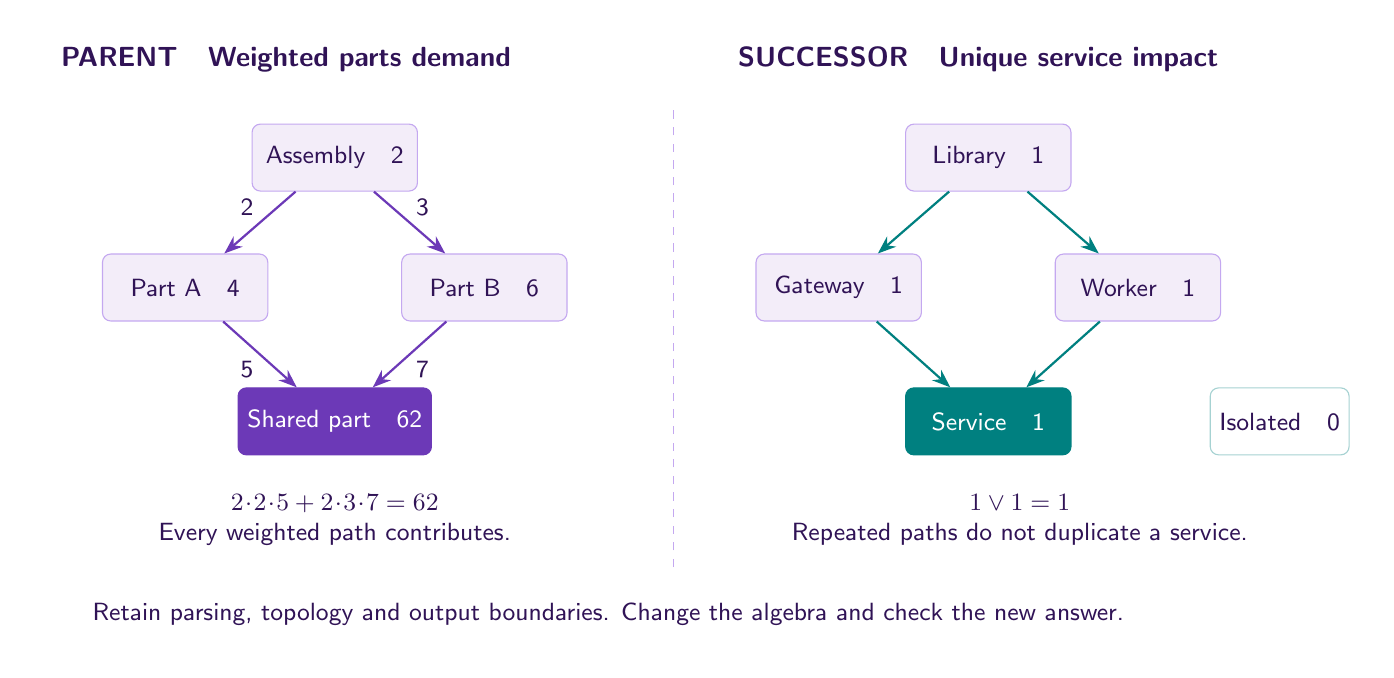
\begin{tikzpicture}[font=\sffamily,>=Stealth,
 nodebox/.style={draw=Lilac,fill=PalePurple,rounded corners=3pt,minimum width=2.1cm,minimum height=.85cm,align=center,font=\sffamily\small,text=DeepPurple},
 outbox/.style={nodebox,fill=RoyalPurple,text=white,draw=RoyalPurple},
 edgelabel/.style={font=\sffamily\small,text=DeepPurple,fill=white,inner sep=2pt}]
\fill[white] (-.4,-1.4) rectangle (16.6,6.5);
\node[anchor=west,text=DeepPurple,font=\sffamily\bfseries] at (-.1,6.1) {PARENT\quad Weighted parts demand};
\node[anchor=west,text=DeepPurple,font=\sffamily\bfseries] at (8.5,6.1) {SUCCESSOR\quad Unique service impact};
\node[nodebox] (a) at (3.5,4.85) {Assembly\quad 2};
\node[nodebox] (b) at (1.6,3.2) {Part A\quad 4};
\node[nodebox] (c) at (5.4,3.2) {Part B\quad 6};
\node[outbox] (d) at (3.5,1.5) {Shared part\quad 62};
\draw[->,RoyalPurple,thick] (a)--node[edgelabel,above left]{2}(b);
\draw[->,RoyalPurple,thick] (a)--node[edgelabel,above right]{3}(c);
\draw[->,RoyalPurple,thick] (b)--node[edgelabel,below left]{5}(d);
\draw[->,RoyalPurple,thick] (c)--node[edgelabel,below right]{7}(d);
\node[align=center,text=DeepPurple,font=\sffamily\small] at (3.5,.25) {$2\!\cdot\!2\!\cdot\!5+2\!\cdot\!3\!\cdot\!7=62$\\Every weighted path contributes.};
\draw[Lilac,dashed] (7.8,-.35)--(7.8,5.45);
\node[nodebox] (lib) at (11.8,4.85) {Library\quad 1};
\node[nodebox] (gateway) at (9.9,3.2) {Gateway\quad 1};
\node[nodebox] (worker) at (13.7,3.2) {Worker\quad 1};
\node[outbox,fill=Teal,draw=Teal] (service) at (11.8,1.5) {Service\quad 1};
\node[nodebox,minimum width=1.5cm,draw=Teal!35,fill=white] (isolate) at (15.5,1.5) {Isolated\quad 0};
\foreach \from/\to in {lib/gateway,lib/worker,gateway/service,worker/service}
 \draw[->,Teal,thick] (\from)--(\to);
\node[align=center,text=DeepPurple,font=\sffamily\small] at (12.2,.25) {$1\lor1=1$\\Repeated paths do not duplicate a service.};
\node[anchor=west,text=DeepPurple,font=\sffamily\small] at (.3,-.95) {Retain parsing, topology and output boundaries. Change the algebra and check the new answer.};
\end{tikzpicture}
}%
\endgroup}%
% End embedded vector

\caption{An illustrative exact diamond makes the semantic change visible. Weighted paths add demand; Boolean paths collapse to one impact per service, with an unreachable service remaining zero. This explains the supplied recurrences, not a newly discovered graph algorithm or a commercial observation.}
\label{fig:algebra}
\end{figure}

\subsection{What the enterprise constructs and retains}

The initial capability combines a validated mission protocol, normalized topological representation, weighted kernel and manifest identifying executable modules and dependencies. The successor retains the protocol and representation machinery and adds the Boolean kernel. Its artifact is an executable asset with a declared operation, inputs, outputs, dependency identities, limits, history and cost. The source grammar and both elementary algorithms are supplied by this research implementation. Compilation selects and assembles supported behavior; it is not an unrestricted language model inventing graph theory.

The common representation is enabling because it separates the dependency structure from the operation performed over that structure. A naive reuse path treats an accepted weighted reduction as evidence for all future reductions. The constructed interface instead names the algebra as part of the current capability and mission contract. A diamond-shaped graph is an essential control: multiple paths increase weighted demand, whereas one reachable target still contributes a single Boolean indicator. A changed kernel requires its own qualification even when parser and normalized representation remain compatible.

The flat-reduction control already supplies exact integer rows and needs neither dependency discovery nor graph construction. It preserves a deliberately useful simpler alternative. Adding all enterprise stages to a task that does not need them can increase work without improving its answer.

\section{Mission-relative revalidation}

\subsection{Historical evidence is not current acceptance}

Represent a capability as
\[
K=(\mathrm{id},\mathrm{program},\mathrm{schema},\mathrm{dependencies},\mathrm{scope},
\mathrm{provenance},\mathrm{cost}).
\]
The source inventory binds the actual bytes used in the declared executable closure. A reusable verification result concerns an immutable generic module and its specified checking obligation. A current proof receipt concerns a particular mission, capability, input, output, policy and evaluator version. Those are different objects. Every descendant starts with \texttt{currentProof:null} and \texttt{authority:[]} while retaining historical evidence as history.

The evaluator may reuse previously discharged generic obligations only under its declared complete identity. It still validates every mission input and compares every mission output against the current reference. It produces a new scope-bound result after that work. Neither a cached module check nor an earlier mission result grants permission to execute a consequential action. This distinction is the essential constraint on making revalidation cheaper.

\begin{proposition}[Conditional equivalence of reused checks]
Suppose a deterministic acceptance procedure consists of generic module checks and mission-specific checks. Suppose a cached generic result was produced by that same checker, its key binds every source, dependency, policy and input on which the result depends, the evaluator controls the cache, and identity comparisons are sound. Replacing an identical generic check by that cached result leaves the procedure's accept/reject outcome unchanged, provided every mission-specific check still executes.
\end{proposition}

\begin{proof}
Each cache hit substitutes the same result the deterministic check would return on the same complete inputs. All other checks and the final decision rule are unchanged. Substitution therefore preserves the decision. The conclusion fails if an omitted dependency changes the check, the cache is corrupted, or a mission-specific obligation is incorrectly classified as generic.
\end{proof}

The proposition describes a trust boundary, not a universal security guarantee. Digest collision resistance and complete dependency declaration are assumptions; hashing does not prove semantic truth. The experiment must test changed identities, wrong algebra, altered outputs and refusal cases rather than use the proposition as a substitute for implementation evidence. A collection of successful tests is not a machine-checked theorem for arbitrary programs.

\subsection{Costs, ablations and the prospective threshold}

The primary finite population contains 48 declared missions: 16 weighted bill-of-materials tasks, 16 remediation-impact tasks, 8 flat reductions and 8 invalid requests. The delivery envelope allows at most 64 nodes, 256 edges and 2,000 output rows; bridge-bound integer outputs and their signed aggregate must have absolute value at most one million. Labels use 1--48 ASCII letters, digits, underscores or hyphens; seed arrays are nonempty, although their amounts may be zero. Internal arithmetic uses exact integers with an explicit digit ceiling. The technical alternative is frozen before scored runs: at least a 50\% reduction in counted reusable verification checks at identical acceptance outcomes, with fresh input/output checking reported separately and elapsed time measured. Satisfying that technical condition alone does not establish genuinely realizable monetary value. A stronger practical-value claim also requires independently established usefulness or task-class feasibility under the declared resource envelope.

The comparisons include the integrated loop with reused generic checks, full replay, rebuilding without inheritance, no construction, a wrong-algebra stage ablation and a supplied deterministic direct specialist. The specialist is a credible software reference for the bounded task, not a recruited human expert. It receives the same mission semantics and is allowed to solve the graph directly. A direct winner is a scientific result.

Let $V_i$ denote the generic verification cost of module identity $i$, let $F_m$ denote fresh mission checking, and let $H_m$ denote identity lookup and framing. For a fixed series of missions, full replay repeatedly pays every applicable $V_i$; reuse pays $V_i$ when the identity is first encountered or validly invalidated. Both pay the fresh checks. The experiment reports these categories separately, alongside construction, productive execution, retries and elapsed time. It does not collapse an operation count, a byte count and a token transfer into one economic unit.

Frozen source and scoring are necessary because a proposer could otherwise optimize a convenient checker or remove failed tasks. The independently implemented reference and scoring definition remain outside the enterprise's editable implementation. Reproduction of the now-public task population checks computational repeatability; it cannot recreate the original temporal separation between construction and held-out evaluation.


\subsection{Prospective correction and independent reference}

The first task generator made its Boolean cases too densely connected: every target was reached. A reference audit exposed this weak contrast before the candidate existed and before any scored run. The complete first version remains in \filename{study/evaluation/prescore-v1/}. Version 2 introduced disconnected targets, zero seeds and mixed reachability while preserving the 48-mission population and the decision metrics. It was frozen at 16:20:18 UTC on 23 October 2026. This is a disclosed pre-scoring protocol correction, not a repair informed by candidate results.

The final task-bank SHA-256 starts \texttt{66635281d0c50dea}; the criteria digest starts \texttt{58dd0ba793d9277e}. Full digests and exact bytes are in \filename{study/evaluation/FREEZE.json}. The evaluator computes weighted answers by independent depth-first path enumeration and impact answers by breadth-first unique reachability. These differ from the candidate's topological recurrence. Both share the specified task semantics, so the agreement is algorithmic cross-checking, not a claim that the specification is independently correct.

The proposer was instructed not to inspect the frozen evaluation directory. The evaluator and candidate occupy separate source namespaces under one research controller. This protects the intended workflow from ordinary edits, but it is not hostile operating-system isolation, a formally verified sandbox, or institutionally independent review. Released task bytes become public; a subsequent rerun is a reproduction run, not a fresh held-out test.

The session-clock freeze labels and raw host timestamps are retained as separate observations because the host clock and session clock differ. Elapsed-time measurements use a monotonic clock. Temporal blindness is described by the recorded workflow and preserved source versions, not inferred from a timestamp string alone.

% END method.tex


% BEGIN architecture.tex
\section{One mission across four execution systems}

\subsection{A thin additive interface}

The harness is a bounded caller around actual repository interfaces \cite{alphasource,managersource,jobssource,fleetsource}. It does not replace the four systems or copy the held enterprise Harness under a new name. The new compiler supplies a small, explicit \texttt{group,amount} reporting boundary that the existing systems can already consume. Every boundary preserves the original mission identity and links its receiver-local identifier to it. The same Alpha project can retain a parent cycle and a distinct successor cycle. Source pins and byte inventories travel with the evidence; the corresponding repository names are not used as a substitute for executing their code.

Alpha creates and runs its native public-data mission, retaining project and mission history. Manager consumes those exact output bytes through its portable API, verifies the row arithmetic and constructs its own unsigned USDC6 plan. Jobs consumes that Manager transfer, builds an unfunded AGIALPHA18 work graph and invokes its existing source adapter. Fleet consumes the Jobs transfer, maps the retained Alpha mission to its fixed worker task, calls the actual local worker function and invokes its separate internal checker. These are existing code paths wrapped by a new adapter; their original source-selection checks remain active.

\begin{table}[htbp]
\centering
\small
\begin{tabularx}{\linewidth}{P{0.14\linewidth}P{0.37\linewidth}Y}
\toprule
\textbf{System} & \textbf{Executed public-source contribution} & \textbf{Boundary and retained limitation}\\
\midrule
AGI ALPHA & \filename{examples/successor-project/engine.mjs}; native project, mission and executor modules & Organizational record, exact integer report and history; bounded public-data grammar.\\
AGIJob-\newline Manager & \filename{site/assets/successor/alpha-project.mjs}; selected-source builder & Consumes Alpha bytes, checks the report and prepares a separate unsigned USDC6 route.\\
AGIJobsv0 & \filename{integrations/alpha-agent/project-transfer.mjs}; source selector & Consumes the Manager envelope; unfunded AGIALPHA18 work graph and fixed-source execution.\\
AGI-Fleet-Linux & \filename{local-runtime/project/transfer.mjs}; \filename{local-runtime/worker.mjs} & Consumes Jobs evidence and invokes local execution/checking functions; no installed Fleet-host qualification.\\
\bottomrule
\end{tabularx}
\caption{Executable contribution by repository. Complete commit pins, exact entry points and imported-source hashes are recorded in the companion runtime audit. These local API executions do not imply production installation or live settlement.}
\label{tab:repositories}
\end{table}

Eight separately recorded delivery-admission tests cover altered mission, output, capability or CSV bytes, semantic refusal, forged candidate authority, bounded queuing, duplicate requests, retry and interruption at the supported boundaries. They use controlled checks before native execution and do not constitute a full native load campaign. The existing source bridge separately has nine passing boundary tests.

The bridge intentionally does not reinterpret all monetary units as one token. Manager's USDC6 plan, Jobs' AGIALPHA18 receiver and Alpha's five-contract settlement route have different interfaces and permissions. An illustrative budget remains unfunded. The new compiler's semantic acceptance is also separate from row aggregation: adding correct rows does not prove that the right graph question produced them. The fresh evaluator binds its result to the exact mission, capability, output, criteria and checker. A downstream transaction can commit that hash; it cannot turn an incorrect scientific result into a correct one.

\subsection{Customer-owned WORLD, POLICY, PROOF and AUTHORITY}

The customer-continuity representation separates four concerns. \textbf{WORLD} contains the graph, observations, source identities and explicit uncertainty about demand and applicability. \textbf{POLICY} declares the mission kind, exact-output rule, resource ceilings and prohibited routes. \textbf{PROOF} contains independently recomputed finite evidence and current scope, with historical results retained separately. \textbf{AUTHORITY} contains an explicit grant for a bounded action. Neither a good prediction nor a successful test supplies the grant.

An exported capsule preserves schema, source manifests, compact outcome history, provenance and the current capability's most-recent run cost fields. Full cumulative cost records remain in the separate evidence companion; the compact workspace is not a complete lineage cost ledger. Restore must recreate executable continuity without treating imported acceptance as current certification. A successor starts with empty current proof and authority, and re-establishes mission-specific checks before the permitted execution step. The symbolic representation backend can be replaced within its contract. The observed Kahn-to-DFS swap receives a fresh mission-output check; broader representation qualification remains a requested obligation rather than an inherited certificate. This study does not contain an actual learned-model-provider exchange, so it cannot establish portability across arbitrary model suppliers.

\begin{figure}[htbp]
\centering
% Embedded editable vector: lineage
\resizebox{.80\linewidth}{!}{%
\begingroup
\microtypesetup{protrusion=false,expansion=false}%
\color{black}\fontsize{10}{12}\selectfont
\def\small{\csname @setfontsize\endcsname\small{9}{11}}%
\def\scriptsize{\csname @setfontsize\endcsname\scriptsize{7}{8}}%
\def\large{\csname @setfontsize\endcsname\large{12}{14}}%
\setlength{\fboxsep}{10pt}%
\definecolor{purple}{HTML}{301356}
\definecolor{lilac}{HTML}{F3EDF9}
\definecolor{green}{HTML}{14634E}
\definecolor{gray}{HTML}{5E5969}
\colorbox{white}{% Standalone-equivalent white padding.
\begin{tikzpicture}[font=\sffamily,>=Latex,line width=.7pt]
\node[anchor=west,text=purple,font=\sffamily\bfseries\large] at (0,1.1) {CAPABILITY SURVIVES. CURRENT PROOF IS REBUILT.};
\node[anchor=west,text=gray,font=\sffamily\small] at (0,.5) {The successor inherits executable means and traceable history.};
\node[draw=purple!40,fill=lilac,rounded corners=4pt,minimum width=5.0cm,minimum height=3.1cm,anchor=north west] (parent) at (0,0) {};
\node[anchor=north west,text=purple,font=\sffamily\bfseries] at (.25,-.25) {Parent mission};
\node[anchor=north west,text width=4.5cm,align=left,font=\sffamily\small] at (.25,-.85) {Executable asset\\Inputs, outputs, dependencies\\Limits and construction cost\\Evidence and provenance};
\node[draw=purple!40,fill=lilac,rounded corners=4pt,minimum width=5.0cm,minimum height=3.1cm,anchor=north west] (child) at (6.7,0) {};
\node[anchor=north west,text=purple,font=\sffamily\bfseries] at (6.95,-.25) {Successor mission};
\node[anchor=north west,text width=4.5cm,align=left,font=\sffamily\small] at (6.95,-.85) {New useful requirement\\Retained compatible means\\Current proof: empty\\Current authority: empty};
\draw[->,purple,thick] (5,-1.55)--node[above,font=\sffamily\scriptsize,align=center]{reuse\\structure}(6.7,-1.55);
\node[draw=green!50,fill=green!5,rounded corners=4pt,minimum width=5.0cm,minimum height=3.1cm,anchor=north west] (check) at (0,-4.3) {};
\node[anchor=north west,text=green,font=\sffamily\bfseries] at (.25,-4.55) {Fresh mission evaluation};
\node[anchor=north west,text width=4.5cm,align=left,font=\sffamily\small] at (.25,-5.13) {Fixed criteria, separate checker\\Candidate and output binding\\Result or retained failure};
\node[draw=purple!40,fill=white,rounded corners=4pt,minimum width=5.0cm,minimum height=3.1cm,anchor=north west] (grant) at (6.7,-4.3) {};
\node[anchor=north west,text=purple,font=\sffamily\bfseries] at (6.95,-4.55) {Authority decision};
\node[anchor=north west,text width=4.5cm,align=left,font=\sffamily\small] at (6.95,-5.13) {Action, budget and expiry\\Accountable permission source\\Stop, revoke and rollback};
\draw[->,purple,thick] (9.2,-3.1)--(9.2,-3.7)--(2.5,-3.7)--(2.5,-4.3);
\node[font=\sffamily\scriptsize,text=gray,fill=white] at (5.85,-3.7) {re-establish current evidence};
\draw[->,green,thick] (5,-5.55)--node[above,font=\sffamily\scriptsize,align=center]{fresh\\receipt}(6.7,-5.55);
\node[anchor=north west,text=gray,text width=11.7cm,font=\sffamily\scriptsize,align=left] at (0,-7.85) {Architectural invariant. Historical evidence helps determine what can be reused; it is never a transfer of present acceptance or permission. Evaluation and authorization remain separately accountable.};
\end{tikzpicture}
}%
\endgroup}%
% End embedded vector

\caption{Inheritance preserves an executable asset and its history. Fresh mission acceptance and a separate bounded authority grant remain necessary. This is the enforced design invariant; individual execution evidence is reported separately.}
\label{fig:lineage}
\end{figure}

The runtime's source inventory hashes regular-file bytes against recorded Git objects, the imported module closure, the caller, Node version, Fleet lockfile and Manager source manifest. This is valuable reproducibility evidence. It is not a complete operating-system security boundary: an adversary controlling the host, undeclared runtime state or the evaluator could violate its assumptions. This research supplies no such privilege expansion to the candidate.

\FloatBarrier
\subsection{The instrumented organizational loop}

The stage names provide an accountability map. Identify records a supported gap and its binding constraint; it explicitly distinguishes the supplied mission family from validated customer demand. Out-Learn inventories exact installed module identities and declared dependencies; graph parsing occurs during execution and capability-gap matching during design. Out-Think replaces a fixed arithmetic interpretation with a graph representation whose algebra is explicit. Out-Design assembles a bounded executable capability with dependencies and verification obligations. Out-Strategise records the experiment-assigned route and budget; flat controls use the supported direct path without constructing a graph capability. Out-Execute invokes the authorized boundary and retains its exact artifacts. Out-Evolve proposes the changed Boolean capability and submits it to independent evaluation before any promotion.

A stage can be skipped when an existing valid artifact meets the current obligation. The justification belongs in the trace. For example, a flat-reduction request should not acquire a graph compiler merely to display all six names. The direct specialist is therefore a substantive comparator, and a full-loop loss is reported as a cost of organization within this envelope. The function names alone make no claim of superiority to humans, beyond-human foresight or autonomous sovereignty.

The experiment separates the proposer, evaluator and authority-enforcement code. This is a real executable division of responsibility inside the research controller, not independent institutions. Promotion must follow proposal, sandbox construction, evaluation and an explicit bounded grant. Rejection, stale source, wrong algebra, invalid input or exhausted limits must leave the proposed artifact unadmitted. Recovery retains the old valid asset and its history; it does not erase failed trials or grant the child its parent's status.

\subsection{What the local journey can and cannot mean}

The beginner journey explains a concrete path: discover the graph capability gap, create a plan, bind the exact work, execute locally, inspect validation, inspect local settlement, retain the asset and attempt a different mission. Each step exposes the useful output, measured cost or unknown cost, next action and proof status. Technical details belong in an optional drawer containing source versions, mission identifiers, permissions and failure evidence. A static result is labeled a replay. A fresh local result is labeled local execution. A read from deployed code is labeled a live read. The existence of a polished screen must not blur these categories.

The local demonstration requires no wallet or gas purchase. Any advanced live preparation is an unsigned intent for a separately authorized user-wallet handoff. No address read, risk attestation, token quote or local receipt authorizes a mainnet transaction. Production native-host qualification, the held Harness review and merge, and held browser/native probes remain outside the completed scope. The new Writer \#4 HTTP interface has its own executed browser acceptance and desktop/mobile visual review, reported below; these checks do not qualify earlier held surfaces or native-host objectives.

% END architecture.tex


% BEGIN results.tex
\section{Executed comparisons}
\label{sec:results}

The initially frozen candidate was evaluated on all 48 missions in three complete repetitions for each of seven variants, giving 1,008 mission executions. A narrowly repaired final version then repeated the same known bank for another 1,008 executions; that confirmation is not a new blinded study. Six variants belong to the predeclared comparison; the old-representation control is explicitly supplementary. Each repetition uses the same finite task population. It is a repeatability and timing observation, not 48 new random draws or an estimate of general enterprise success.

The original candidate source-inventory digest starts \texttt{cc9b237f8ebf500f}; the final version starts \texttt{71fed4b4befecc4f}. The evaluator digest starts \texttt{7eebf95de7ff0b36}; the qualifier is \texttt{df6d832dec259079}; the runner is \texttt{3ed31a743fd01c61}. Full identities, every scored failure and all run metrics are retained separately in \filename{study/results/scored-v1/} and \filename{study/results/scored-v2/}. Source was fixed within each campaign. The tables below use the final known-bank confirmation, with original differences disclosed.

\subsection{The prospective technical condition passes}

The integrated reuse route accepts all 40 valid missions and rejects all eight invalid requests in every repetition. Full replay, rebuilding without inheritance and the direct specialist have identical correct decisions. Reuse executes 64 generic qualification cases per 48-mission trial, compared with 1,600 under full replay: a 96.0\% reduction. This exceeds the prospectively declared 50\% technical threshold while preserving the same acceptance decisions and fresh mission checks.

The reduction concerns finite cases, not universal program proofs. Qualification uses 1,733 independent-reference steps under reuse and 44,416 under full replay. Fresh scoring and receipt generation add 3,624 reference steps to each route. Including those fresh steps, the corresponding reference-work totals are 5,357 and 48,040, an 88.85\% reduction in that single counted category. Source identity and hashing work remain: candidate hashing is 2,113,989 bytes and qualification hashing is 1,232,000 bytes for each of these two routes. The study does not report a 96\% reduction in all computation, all latency or money.

\begin{table}[htbp]
\centering
\small
\begin{tabularx}{\linewidth}{Yrrrr}
\toprule
\textbf{Variant} & \textbf{Accepted /40} & \textbf{Invalid /8} & \textbf{Cases} & \textbf{Events}\\
\midrule
Integrated reuse & 40 & 8 & 64 & 9,048\\
Full replay & 40 & 8 & 1,600 & 9,048\\
No inheritance & 40 & 8 & 1,600 & 9,133\\
No construction & 8 & 8 & 8 & 572\\
Old algebra & 28 & 8 & 64 & 9,048\\
Direct specialist & 40 & 8 & 64 & 8,562\\
Old representation$^*$ & 11 & 8 & 64 & 8,090\\
\bottomrule
\end{tabularx}
\caption{Outcomes and work per 48-mission trial; identical in all three repetitions. ``Invalid'' counts correctly rejected requests. ``Cases'' counts generic qualification cases. ``Events'' counts candidate instrumentation events, not processor instructions or dollars. $^*$Supplementary control, outside the six predeclared variants.}
\label{tab:outcomes}
\end{table}

\begin{figure}[htbp]
\centering
% Embedded editable vector: comparison
\resizebox{\linewidth}{!}{%
\begingroup
\microtypesetup{protrusion=false,expansion=false}%
\color{black}\fontsize{10}{12}\selectfont
\def\small{\csname @setfontsize\endcsname\small{9}{11}}%
\def\scriptsize{\csname @setfontsize\endcsname\scriptsize{7}{8}}%
\def\large{\csname @setfontsize\endcsname\large{12}{14}}%
\setlength{\fboxsep}{5pt}%
\definecolor{DeepPurple}{HTML}{301356}
\definecolor{RoyalPurple}{HTML}{6C39B7}
\definecolor{Lilac}{HTML}{C4A8F0}
\definecolor{Muted}{HTML}{81788C}
\definecolor{Teal}{HTML}{14634E}
\definecolor{Grid}{HTML}{EAE4F0}
\colorbox{white}{% Standalone-equivalent white padding.
\begin{tikzpicture}[font=\sffamily]
\node[anchor=west,text=DeepPurple,font=\sffamily\bfseries] at (-.1,6.0) {A\quad Generic qualification cases};
\node[anchor=west,text=DeepPurple,font=\sffamily\bfseries] at (8.6,6.0) {B\quad Wall time per 48-mission trial};
\begin{axis}[at={(0,0)},width=8.4cm,height=6.1cm,ybar,bar width=19pt,
 xmin=-.6,xmax=3.6,ymin=0,ymax=1800,xtick={0,1,2,3},xticklabels={Reuse,Replay,Rebuild,Direct},
 ytick={0,400,800,1200,1600},ymajorgrids,grid style={Grid},axis line style={Muted!50},
 tick label style={font=\sffamily\small},label style={font=\sffamily\small},
 ylabel={Finite module cases},enlarge x limits=false,
 nodes near coords,nodes near coords style={font=\sffamily\small,text=DeepPurple},
 every axis plot/.append style={draw=none},clip=false]
\addplot[fill=RoyalPurple,bar shift=0pt] coordinates {(0,64)};
\addplot[fill=Muted,bar shift=0pt] coordinates {(1,1600)};
\addplot[fill=Lilac,bar shift=0pt] coordinates {(2,1600)};
\addplot[fill=Teal,bar shift=0pt] coordinates {(3,64)};
\end{axis}
\begin{axis}[at={(8.7cm,0)},width=8.4cm,height=6.1cm,
 xmin=-.6,xmax=3.6,ymin=0,ymax=270,xtick={0,1,2,3},xticklabels={Reuse,Replay,Rebuild,Direct},
 ytick={0,50,100,150,200,250},ymajorgrids,grid style={Grid},axis line style={Muted!50},
 tick label style={font=\sffamily\small},label style={font=\sffamily\small},ylabel={Milliseconds},
 enlarge x limits=false,clip=false]
\addplot[only marks,mark=*,mark size=3pt,color=RoyalPurple,thick,error bars/.cd,y dir=both,y explicit,error mark options={rotate=90,mark size=4pt}] coordinates {(0,59.867163) += (0,51.755841) -= (0,4.391675)};
\addplot[only marks,mark=*,mark size=3pt,color=Muted,thick,error bars/.cd,y dir=both,y explicit,error mark options={rotate=90,mark size=4pt}] coordinates {(1,163.225064) += (0,83.773235) -= (0,4.291234)};
\addplot[only marks,mark=*,mark size=3pt,color=Lilac,thick,error bars/.cd,y dir=both,y explicit,error mark options={rotate=90,mark size=4pt}] coordinates {(2,164.471672) += (0,34.549767) -= (0,11.203472)};
\addplot[only marks,mark=*,mark size=3pt,color=Teal,thick,error bars/.cd,y dir=both,y explicit,error mark options={rotate=90,mark size=4pt}] coordinates {(3,54.920640) += (0,13.487600) -= (0,8.212295)};
\end{axis}
\node[anchor=west,text=DeepPurple,font=\sffamily\small] at (.45,-1.15) {All four: 40/40 valid missions accepted; 8/8 invalid requests rejected.};
\node[anchor=west,text=Muted,font=\sffamily\small] at (.45,-1.65) {Fresh mission checks remain. Points: median; whiskers: observed min--max, 3 trials.};
\end{tikzpicture}
}%
\endgroup}%
% End embedded vector

\caption{Final known-bank confirmation at matched exact acceptance. Generic finite qualification cases fall under reuse. Wall-time ranges are descriptive observations; the specialist uses fewer candidate events and less pooled CPU. Editable vector source and exact figure data accompany the paper.}
\label{fig:comparison}
\end{figure}

\subsection{A changed algebra is necessary within the declared grammar}

Without capability construction, the existing flat route accepts the eight flat controls and refuses all 32 graph tasks. The complete route accepts all 40 valid tasks. Thus finite useful-input coverage rises from 20\% to 100\% within this supplied task population. This is an expansion relative to the native flat grammar, not evidence that no existing solver could answer the graphs. The direct specialist also reaches 100\%.

Retaining the old weighted algebra accepts all 16 bill-of-materials tasks and all eight flat controls, but only four of the 16 remediation tasks. Twelve impact answers fail the independent semantic check. The four coincidentally correct cases prevent an exaggerated claim that every wrong-algebra attempt must fail. The supplementary old-representation control accepts no bill-of-materials tasks, three remediation tasks and the eight flat controls. These controls show why preserving the correct graph structure and changing its interpretation matter to this population.

The successor retains the protocol, graph representation, normalization and weighted capability as history and adds a Boolean executable kernel when that grammar is first needed. Later remediation missions reuse that new kernel. The first construction event and later warm-use events are separate trace entries. The original exported successor at remediation mission 01 is already a warm reuse after the Boolean grammar was added; it is not relabeled as the construction event. The connected flagship instead starts a fresh parent and then selects remediation mission 03 to expose mixed reachable and unreachable targets. That illustrative selection was made after scoring and is not a separately blinded sample. Every returned candidate still has empty current proof and authority, including successful ones. Acceptance is issued externally for its actual current input and output.

\subsection{The specialist remains a serious alternative}

The direct specialist needs 8,562 candidate events per trial, compared with 9,048 for integrated reuse, and performs no typed-IR construction. Reuse records 227 construction events; rebuilding records 312. The specialist also has lower pooled CPU time across the three trials: 195.9 milliseconds including user and system CPU, versus 284.3 milliseconds for reuse. Both accept the same valid tasks and reject the same invalid tasks. The integrated route therefore does not establish a general efficiency advantage over direct expert software.

\begin{table}[htbp]
\centering
\small
\begin{tabularx}{\linewidth}{Yrrr}
\toprule
\textbf{Variant} & \textbf{Median ms} & \textbf{Min--max ms} & \textbf{Pooled CPU ms}\\
\midrule
Integrated reuse & 59.87 & 55.48--111.62 & 284.33\\
Full replay & 163.23 & 158.93--247.00 & 667.41\\
No inheritance & 164.47 & 153.27--199.02 & 619.44\\
No construction & 27.66 & 27.61--33.53 & 95.35\\
Old algebra & 57.53 & 54.51--64.42 & 194.02\\
Direct specialist & 54.92 & 46.71--68.41 & 195.86\\
Old representation$^*$ & 65.47 & 59.73--99.63 & 242.82\\
\bottomrule
\end{tabularx}
\caption{Wall time is per complete 48-mission trial; the range and median use three repetitions. CPU sums user and system time across all three trials, so it has a different denominator. Low-quality ablations are retained rather than compared as equivalent services. These are local microbenchmarks.}
\label{tab:timing}
\end{table}

The direct specialist wins median wall time in the final confirmation: 54.92 versus 59.87 milliseconds. The original campaign had the opposite order, with reuse at 60.08 and direct at 72.64 milliseconds. Its replay and rebuild medians were 197.40 and 229.86 milliseconds. Both full records remain available. Three timings per version are insufficient for a universal speed claim, and the reversal demonstrates why warmup, scheduling and accounting overhead matter at this scale. The clear measured contribution is avoiding repeated generic qualification compared with full replay. A buyer-facing claim would additionally need an established useful workload and a complete cost comparison.

The US\$100-to-US\$10,000 target remains unproven. The technical threshold passes, but the stronger practical-value condition requires independently established usefulness or task-class feasibility beyond these authored synthetic examples. No commercial return is inferred from the counted-work result.


\subsection{A retained lineage defect and a known-bank repair}

An independent review after the first scored campaign found a provenance defect: unchanged capability content could be assigned its own identifier as its parent. Exact mission outputs still passed, but the lineage record was wrong. The final repair preserves the earlier parent when the content identifier is unchanged and uses the previous capability identifier only when content changes. It changes no graph algorithm or task population. A new development test follows three generations; all twelve public development checks pass.

The complete original seven-module source snapshot, development evidence and scored results are retained under \filename{study/results/scored-v1/candidate-source/}. The repaired candidate is re-frozen before its full known-bank confirmation. Acceptance, qualification-case counts, reference work and candidate event counts remain unchanged, while timing and hashed byte counts differ. This distinction prevents a repaired release from being presented as if its exact bytes had been the original unseen candidate. It also shows that correct task answers alone do not validate all claims about an inherited asset.

\subsection{The connected local flagship}

The final two-mission source journey executes the weighted parent and a fresh Boolean successor through every repository. Parent target amounts are 25, 25, 25 and 50, totaling 125. Successor amounts are 1, 0, 1 and 0, totaling 2. Every group matches the separately computed semantic artifact; aggregate agreement alone is not used as acceptance. Alpha retains one project with two cycles, and the original mission identifiers survive in the nested Manager, Jobs and Fleet transfers. The child's construction ledger retains four modules and adds the Boolean kernel, with a genuine parent identity.

The pair takes 5,650.50 milliseconds locally, including the four-source execution boundary. That is a different operation from the small compiler microbenchmark and should not be compared as the same latency. The bridge records no financial transfer, no installed-host admission and no tested process isolation. The exact artifact-to-local-EVM join is reported with its own receipt. The standalone bridge's \texttt{settlement:not-connected} field remains accurate for that adapter rather than being overwritten to imply that it settles funds itself.

% END results.tex


% BEGIN load.tex
\section{Load, control and measured stage costs}

\subsection{The tested load envelope}

The final source is exercised at volumes 8, 32 and 128, with one or two local Node worker threads and two repetitions per setting. All 672 submitted valid tasks are accepted and exactly correct, with no run intervention and zero observed failure rate. This is an execution-volume test over reused finite tasks. It does not add new mission classes, measure physical Fleet machines or qualify the full four-repository path at those volumes.

\begin{table}[htbp]
\centering
\small
\setlength{\tabcolsep}{4pt}
\begin{tabularx}{\linewidth}{rrYYYY}
\toprule
\textbf{Workers} & \textbf{Tasks} & \textbf{Wall ms} & \textbf{Tasks/s} & \textbf{p95 ms} & \textbf{Cases}\\
\midrule
1 & 8 & 95.4--109.3 & 73.2--83.9 & 94.0--104.1 & 48\\
1 & 32 & 123.2--133.9 & 239.0--259.8 & 119.9--130.8 & 64\\
1 & 128 & 229.3--443.9 & 288.4--558.1 & 216.9--429.8 & 64\\
2 & 8 & 81.0--82.7 & 96.7--98.8 & 80.1--81.2 & 96\\
2 & 32 & 105.7--107.6 & 297.5--302.9 & 101.6--105.4 & 128\\
2 & 128 & 173.3--183.4 & 697.9--738.7 & 162.8--175.7 & 128\\
\bottomrule
\end{tabularx}
\caption{Ranges over two repetitions at each declared setting. Wall time includes worker startup; task latency includes queue waiting. Cases are generic qualification cases per run. Every row has exact acceptance of all submitted valid tasks and zero observed failures. Source: load summary and per-run receipts.}
\label{tab:load}
\end{table}

Two workers improve observed throughput in this small envelope while duplicating worker-local qualification: the full 128-task load uses 128 cases rather than 64. More concurrent work therefore does not automatically reduce total checking. Candidate events per accepted result are 262.75 at volume 8, 259.72 at 32 and 217.30 at 128 in either concurrency setting. These different averages also reflect which finite tasks occur at each volume. Cost in dollars per accepted result remains unknown. Maximum reported process RSS across these runs is 91,276 KiB; this is a process observation, not an installation memory guarantee.

Zero human interventions means no manual change was made during these short automatic runs. It excludes design, setup, debugging, external review and later operation. Both worker startup and queue waiting matter here; a warm kernel throughput number would answer a different question. The useful envelope is bounded to two local workers, a queue capacity of at most 256 records and the declared graph limits. No production availability, geographically distributed execution or asymptotic scale claim follows.

\subsection{Nine executable control checks}

All nine separately recorded queue/checker control tests pass. They exercise duplicate submissions returning the same completed result, refusal of changed input under a reused identifier, one retained transient failure followed by a bounded retry, a kill switch and restoration that require fresh execution, rejection of the review role's execution request, and the volume ceiling. Verification controls force requalification after a context change, reject changed source bytes pretending to be already-loaded functions, reject stale input or altered answers, and reject inherited permission. Export/restore with the symbolic Kahn-to-DFS change preserves history and clears current state.

The count is nine test cases, some containing several assertions; it must not be added to 38 contract tests or twelve public development checks and labeled one independent validation study. All operate under the same controller. The exact failure history and interruption outcomes are retained in \filename{study/results/control-tests.json}. Neither this suite nor the load test executes any held native or browser probe.

\subsection{Each stage has a visible denominator}

Table~\ref{tab:stagecost} reports the final fresh-parent/Boolean-child illustration, selected after scoring to make the changed semantics visible. Both candidates are complete and externally accepted. The parent's candidate wall time is 6.94 milliseconds and the child's is 2.67 milliseconds in that particular run; these are descriptive single observations before the much slower four-repository journey. They are not a claim that successors are always faster.

\begin{table}[htbp]
\centering
\small
\begin{tabularx}{\linewidth}{Yrrrr}
\toprule
\textbf{Function} & \textbf{Parent events} & \textbf{Child events} & \textbf{Parent bytes} & \textbf{Child bytes}\\
\midrule
Identify & 1 & 1 & 597 & 762\\
Out-Learn & 7 & 7 & 41,941 & 41,941\\
Out-Think & 1 & 1 & 0 & 0\\
Out-Design & 7 & 11 & 1,506 & 2,205\\
Out-Strategise & 1 & 1 & 0 & 0\\
Out-Execute & 178 & 244 & 922 & 1,126\\
Out-Evolve & 1 & 1 & 0 & 0\\
\midrule
Total & 196 & 266 & 44,966 & 46,034\\
\bottomrule
\end{tabularx}
\caption{Instrumented candidate events and bytes passed to hashing, from the two retained candidate receipts. A zero means zero in that counter, not zero elapsed work or zero financial cost. Independent qualification, semantic checking, source-bound integration, EVM execution and engineering costs are separate.}
\label{tab:stagecost}
\end{table}

The child's Out-Design trace names the Boolean kernel as added and four modules as retained. The trace records inputs, outputs, stage status and the reason for any skip. On flat controls, representation construction and successor proposal are skipped because they add no useful capability. Variant selection in Out-Strategise is assigned by the experiment; the trace makes that limitation visible rather than imply that an autonomous business optimizer discovered the best route.

% END load.tex


% BEGIN contracts.tex
\section{Five contracts, five different responsibilities}

The five Alpha contracts were inspected at commit \texttt{9cb90e8c189f146e}. Their sources, shared token wrapper, constants, dependency lock, compiler policy and Hardhat configuration \cite{alphasource} match the recorded deployed-source reference \texttt{c0fc5217e364a39a} in ten exact file comparisons. This establishes those comparisons, not identity of every file in both repository trees. All exact paths, source hashes and read-only observations are included in \filename{evidence/contracts/}.

\subsection{The actual lifecycle}

AscensionAccess combines a canonical live ENS name with an unexpired governor admission. The supported names distinguish Business, Agent and Validator roles. A token balance is not an admission decision. NovaSeed then preserves an immutable genome containing a capsule commitment, a bounded job-plan root and count, an evidence commitment, creator and optional parent lineage. The metadata URI is stored separately by its ERC-721 implementation. The parent must be owned by the minting account. Sealing an NFT does not encrypt its capsule, validate its plan or transfer intellectual property or equity.

RiskOracle records identifiable staked validator attestations. It requires current access, a minimum stake and a suitable open review. It excludes both the current seed owner and original creator from review, including after a transfer, and rejects duplicate votes; its \texttt{green} decision depends on quorum, bounded risk and approved policy. The contract records judgments supplied by validators. It is not a learned risk model and does not itself prove that a business will succeed.

MARK governs a reserve-funded campaign associated with the seed. It supports funding-phase purchases, redemptions and lot transfers; blooming ends that trading phase. Subsequent spending is restricted to committed job-plan leaves and current conditions. JobMarket escrows the bounded work, accepts eligible bids, assigns a worker, records a submitted artifact hash, collects distinct validator votes and settles or recovers funds according to its rules. The five functions are complementary; making an unnecessary transaction just to touch another contract would not improve the evidence.

\begin{table}[htbp]
\centering
\small
\begin{tabularx}{\linewidth}{P{0.19\linewidth}Y Y}
\toprule
\textbf{Contract} & \textbf{Supported user benefit and entry points} & \textbf{Evidence, dependencies and limits}\\
\midrule
AscensionAccess & Attributable, expiring entry: \texttt{register}, \texttt{setAdmission}, \texttt{eligible}. & ENS/NameWrapper and governor; \texttt{Registered}, \texttt{AdmissionSet}. No automatic token-gated access.\\
NovaSeed & Immutable plan and parent record: \texttt{seal}, \texttt{plan}, \texttt{creatorOf}. & Eligible Business, 1--128 jobs, nonzero commitments, owned parent; \texttt{SeedSealed}. No inherited certification.\\
RiskOracle & Staked risk/policy review and capacity: \texttt{deposit}, \texttt{openReview}, \texttt{attest}, \texttt{green}. & Eligible distinct validators, captured review and current ownership; risk, stake and availability events. No autonomous forecast.\\
JobMarket & Bounded escrow, exact-artifact voting and settlement: \texttt{postFromSeed}, \texttt{bid}, \texttt{award}, \texttt{submit}, \texttt{validate}. & Access, oracle, canonical token, opted-in committee; posted, delivered, payout and closure events. No semantic checker in Solidity.\\
MARK & Plan-constrained reserve funding and recovery: \texttt{open}, \texttt{buy}, \texttt{bloom}, \texttt{route}, \texttt{collect}, \texttt{close}, \texttt{reclaim}. & Green seed, owner and Business conditions, Merkle proof; funding, routing and capital-return events. No proven demand or guaranteed return.\\
\bottomrule
\end{tabularx}
\caption{Contract-to-user-benefit map, preserving source-defined functional differences. Exact signatures, addresses, roles, dependencies and ABI comparison are supplied in the contract companion.}
\label{tab:contracts}
\end{table}

A FusionPlan is an off-chain bounded list of exact job specifications committed as a Merkle root in NovaSeed. The existing JavaScript plan builder and Python Ascension compiler implement the corresponding plan encoding. MARK verifies the index-specific leaf and rejects altered specifications or replayed leaves. JobMarket's stored \texttt{specHash} uses index zero. The integration must therefore retain both the plan-index leaf and the market specification hash; treating them as interchangeable would lose an important boundary.

\subsection{Concrete token utility and terminal outcomes}

The canonical \$AGIALPHA token has 18 decimals. The verified source supports validator stake, worker collateral, MARK reserves, job escrow, worker and validator rewards, burns, slashing and refunds. RiskOracle's observed minimum stake is 10 tokens, quorum is two and maximum accepted risk is 2,000 basis points. JobMarket uses three distinct opted-in validators excluding the business, client and worker, with two votes sufficient for the corresponding terminal decision. Agent collateral is the greater of the minimum stake and one tenth of the bounty.

Accepted work uses a five-percent validator-fee rule, divided with integer flooring between the two approving validators; the worker receives the remaining agreed price. Each gross payout burns one percent, with integer flooring. In the retained local 80-token accepted-price fixture, worker gross is 76, worker net is 75.24, validators receive a combined net 3.96 and total burn is 0.8. A 158-token funded campaign with 100 in escrow and a final accepted price of 80 returns 78 unused tokens. These are quantities in a disposable local test-token ledger. They are not payments by a customer, dollars, live revenue or economic profit.

Rejection and missed delivery can slash worker collateral; a delivered job that lacks review quorum instead refunds and unlocks without that slash. Exact-balance-delta checks and total-supply burn checks reject accounting substitutes that merely emit a plausible event. The USDC6 path in AGIJobManager remains separate, including its distinct naming conventions. Nothing in the demonstration converts it into \$AGIALPHA or claims that an Alpha-local test deploys the other repositories' monetary routes.

\subsection{The new artifacts are joined to the local lifecycle}

The final flagship carries both exact scientific artifacts into one disposable chain, with the same five deployed local contract instances. The parent artifact digest starts \texttt{d17d45bb353d1d8c}; the successor starts \texttt{86926380eb154463}. These match the semantic acceptance and all four repository-transfer bindings. The EVM adapter captures the artifact, input, proof, candidate and frozen source-manifest bytes, verifies the frozen source and receipt anchors, recomputes candidate and artifact identities, and reruns the frozen checker in a fresh process for each mission before settlement. It does not trust a candidate's claim that a check passed.

The shared fixture records 70 setup transactions once, followed by 16 lifecycle transactions for each mission. Two jobs settle. The successor seed has identifier 2 and an on-chain parent of seed 1, checked by readback. The captured child artifact declares null current proof and empty authority; these are off-chain artifact fields, not NovaSeed storage. A separate accepted checker receipt already exists before sealing. On-chain readback shows that the child has no risk approval before its own review, after which it obtains exact-artifact votes and local settlement. The session takes 1.386 seconds and records 5,137,741 lifecycle gas units, in addition to 15,015,015 setup gas units. Gas is not converted into a fiat expense because no live transaction or gas purchase occurs.

Each mission uses 158 mock tokens and satisfies the same 75.24 worker, 3.96 validators, 0.8 burn and 78 refund conservation equation. The pair therefore records 316 mock tokens funded and two independent job settlements, not 316 dollars of business revenue. Full receipts are \filename{evidence/contracts/writer4-parent-lifecycle.json} and \filename{writer4-successor-lifecycle.json}; the parent file embeds the child receipt as well, so the same transactions must not be counted twice.

The actual temporal sequence is bounded evidence replay: the graph artifacts and four-source deliveries are computed first, then the local EVM posts, assigns and settles jobs against those exact precomputed bytes after fresh checking. A production dispatcher in which a live JobMarket award triggers an installed Fleet worker is not implemented here. This ordering still tests the artifact boundary and real local contract lifecycle, but it must not be described as a live autonomous market.

\begin{figure}[htbp]
\centering
% Embedded editable vector: accounting
\resizebox{\linewidth}{!}{%
\begingroup
\microtypesetup{protrusion=false,expansion=false}%
\color{black}\fontsize{10}{12}\selectfont
\def\small{\csname @setfontsize\endcsname\small{9}{11}}%
\def\scriptsize{\csname @setfontsize\endcsname\scriptsize{7}{8}}%
\def\large{\csname @setfontsize\endcsname\large{12}{14}}%
\setlength{\fboxsep}{6pt}%
\definecolor{DeepPurple}{HTML}{301356}
\definecolor{RoyalPurple}{HTML}{6C39B7}
\definecolor{Lilac}{HTML}{C4A8F0}
\definecolor{Teal}{HTML}{14634E}
\definecolor{Coral}{HTML}{B74354}
\colorbox{white}{% Standalone-equivalent white padding.
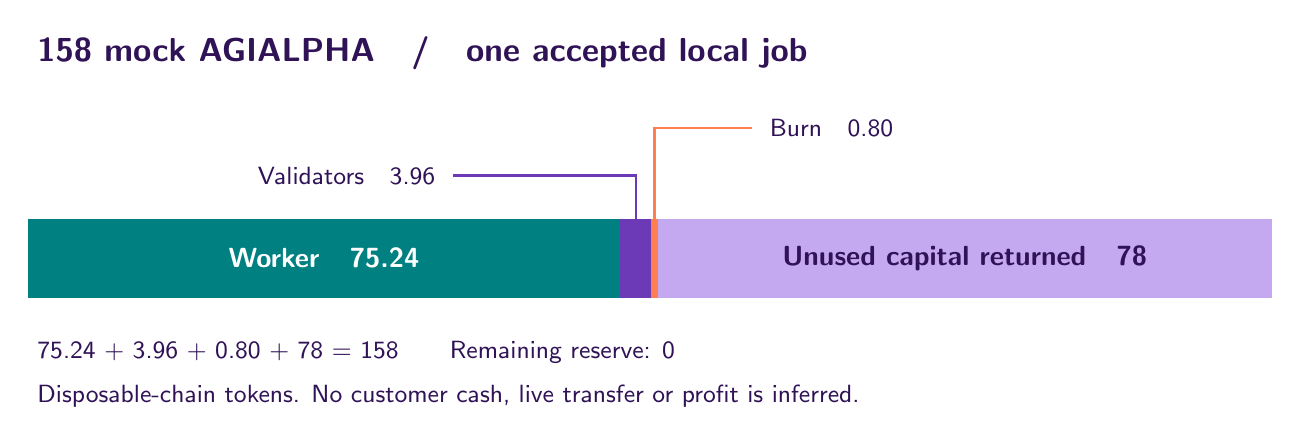
\begin{tikzpicture}[font=\sffamily,x=.1cm,y=1cm,>=Stealth]
\node[anchor=west,text=DeepPurple,font=\sffamily\bfseries\large] at (0,3.1) {158 mock AGIALPHA\quad /\quad one accepted local job};
\fill[Teal] (0,0) rectangle (75.24,1);
\fill[RoyalPurple] (75.24,0) rectangle (79.2,1);
\fill[Coral] (79.2,0) rectangle (80,1);
\fill[Lilac] (80,0) rectangle (158,1);
\node[text=white,align=center,font=\sffamily\bfseries] at (37.62,.5) {Worker\quad 75.24};
\node[text=DeepPurple,align=center,font=\sffamily\bfseries] at (119,.5) {Unused capital returned\quad 78};
\draw[RoyalPurple,thick] (77.22,1)--(77.22,1.55)--(54,1.55);
\node[anchor=east,text=DeepPurple,font=\sffamily\small] at (53,1.55) {Validators\quad 3.96};
\draw[Coral,thick] (79.6,1)--(79.6,2.15)--(92,2.15);
\node[anchor=west,text=DeepPurple,font=\sffamily\small] at (93,2.15) {Burn\quad 0.80};
\node[anchor=west,text=DeepPurple,font=\sffamily\small] at (0,-.7) {75.24 + 3.96 + 0.80 + 78 = 158\qquad Remaining reserve: 0};
\node[anchor=west,text=DeepPurple,font=\sffamily\small] at (0,-1.25) {Disposable-chain tokens. No customer cash, live transfer or profit is inferred.};
\end{tikzpicture}
}%
\endgroup}%
% End embedded vector

\caption{Actual local fixture accounting for one accepted job; the final flagship settles two such jobs. Every amount is mock \$AGIALPHA in a disposable local EVM. The preserved USDC6 route is separate. No bar denotes cash received or profit.}
\label{fig:accounting}
\end{figure}

\subsection{Executed tests and live read-only observations}

The unchanged contract-only suite compiled 55 Solidity files and passed 33 tests in an unforked in-process Hardhat EVM. Five additional existing Python/native settlement-adapter tests passed with the repository's hash-locked lean dependency set, giving 38 distinct tests. Those additional tests cover plan equivalence, exact-delivery settlement, a paid negative evaluation without candidate admission and the missing-quorum refund path. The older native allocation demonstration generated 18 local-EVM transaction receipts and passed its eight stated checks. That older allocation run remains a separate predecessor fixture, not evidence of the new graph contribution.

The negative paths include unauthorized and cross-wired roles, expired names or admissions, self-review, inadequate stake, duplicate risk votes, denied policy, changed Merkle specifications, replay, unbudgeted jobs, conflicting or unavailable committees, invalid bids, wrong artifact hashes, insufficient votes, eligibility lost after a vote, missed delivery, no review quorum, slippage, funding limits, transferred seeds and rounding or dust recovery. These concrete tests establish bounded source behavior. They are not an independent organizational security audit. Separately, 17 actual-artifact byte-gate controls pass, including cross-mission proof replay, changed source anchors, inherited proof or permission, forged checker objects and a self-consistent altered output with a false accepted flag. A different agent also checks 19 handcrafted unscored semantic and refusal cases without inspecting the held-out bank; all pass. Those are separate logical reviews under one controller, retained in the companion, not additional contract-lifecycle tests.

A fresh read-only Ethereum observation at finalized block 26,256,334 (23 October 2026, 16:05:54--16:05:57 UTC) found all five runtime code hashes equal to the retained 18 October record. Twenty-eight owner, dependency and parameter getters were unchanged; The NovaSeed and JobMarket \texttt{nextId} getters both returned zero; the first mint increments the identifier to one. Official Etherscan ABI objects were structurally equal to the five locally compiled ABIs. Their raw serialization hashes differed from the earlier record's ABI hash fields, whose original hashing envelope was unavailable; historical byte-for-byte ABI reconciliation is therefore not claimed.

The five inspected ABIs expose direct contracts and one-time bindings, with no upgrade/proxy entry point. This observation does not audit all external token, ENS, controller or proxy authority. Neither unchanged deployed bytecode nor a live getter establishes that an off-chain worker, validator committee or commercial market is operating. The read grants no authority and sends no transaction.

% END contracts.tex


% BEGIN coverage.tex
\section{Coverage, accountability and honest gaps}

The coverage unit is an executed function with a recorded artifact and a check, not a logo, role label or screenshot. Tables~\ref{tab:stagecoverage} and~\ref{tab:rolecoverage} distinguish the bounded adapter from broader organizational claims. A check of the final graph answer does not independently validate a claim that the planner chose the best business. Local contract signers are distinct accounts under one controller, not independent firms. Deployed bytecode read-only verification is separately recorded and does not deploy the new harness.

\begin{longtable}{P{0.17\linewidth}P{0.36\linewidth}P{0.39\linewidth}}
\caption{Stage-to-evidence map. All candidate stages record status, input/output references, instrumented operations, hash bytes and failure details; justified skips are explicit. Independent checking applies to declared computational obligations.}\label{tab:stagecoverage}\\
\toprule
\textbf{Stage} & \textbf{Implementation and persistent output} & \textbf{Connected scope and remaining gap}\\
\midrule
\endfirsthead
\toprule
\textbf{Stage} & \textbf{Implementation and persistent output} & \textbf{Connected scope and remaining gap}\\
\midrule
\endhead
Identify & \filename{compiler.mjs}: mission schema, identity, input digest, demand status and binding constraint; existing Alpha discovery brief. & Supplied mission need is explicit; external customer demand and autonomous opportunity discovery remain unvalidated.\\
Out-Learn & \filename{sourceManifest} in \filename{compiler.mjs}: exact installed-module catalog; \filename{protocol.mjs}: bounded meter. & Acquires source and structural information without model calls. It does not acquire a new physical measurement or prove economic advantage.\\
Out-Think & \filename{representation.mjs}: parser, canonical graph and topological order; trace records selected algebra and invariants. & New graph representation preserves paths and multiplicity; fresh external reference checks outputs. Broader representation invention is outside the supplied grammar.\\
Out-Design & \filename{capabilityFor}, \filename{programFor}, \filename{executeProgram}: typed IR, module hashes, retained/added/changed ledger. & Constructs an executable arrangement of declared modules; not unrestricted source synthesis. Candidate cannot certify itself.\\
Out-Strategise & \filename{compiler.mjs}: route and budget record; direct, constructed and ablation variants. & Experiment assigns the compared route. It measures alternatives but does not establish an autonomous optimal strategy selector.\\
Out-Execute & Exact kernels and normalizer; four-repository \filename{source-bridge.mjs} and \filename{mission-delivery.mjs}; fresh evaluator artifact. & Actual existing public APIs and fixed Fleet function execute locally. Installed-host, production-market and live financial execution remain outside scope.\\
Out-Evolve & \filename{createWorkspace}, changed Boolean program, lineage/export/restore; external qualification request. & A distinct supplied algebra becomes available in the child; fresh evaluation and authority remain required. No open-ended recursive improvement claim.\\
\bottomrule
\end{longtable}

Candidate paths in this table are relative to \filename{study/enterprise/}; the source bridge and delivery adapter live under \filename{study/integration/}. The trace does not charge engineering effort or hidden authoring time as zero: the stage meter counts operations and hash bytes only. Stage costs cannot be relabeled as complete enterprise monetary costs. An aborted stage retains its failure in the result, and incomplete output is not publishable as an accepted artifact.

\begin{longtable}{P{0.18\linewidth}P{0.36\linewidth}P{0.38\linewidth}}
\caption{Ascension role coverage. ``Adapter'' means this bounded implementation performs part of the responsibility; it does not establish that a separately named autonomous agent was executed.}\label{tab:rolecoverage}\\
\toprule
\textbf{Role} & \textbf{Actual mechanism and evidence} & \textbf{Status and scope}\\
\midrule
\endfirsthead
\toprule
\textbf{Role} & \textbf{Actual mechanism and evidence} & \textbf{Status and scope}\\
\midrule
\endhead
Insight & Alpha \filename{examples/alpha-discovery/engine.mjs}: opportunity brief, alternatives, evidence and gaps. & Existing module connected and executed; supplied illustrative opportunity. A named autonomous Insight process and validated demand are missing.\\
Nova-Seeds & \filename{NovaSeed.sol}; existing exact plan compiler; immutable seed, capsule, plan and parent commitments. & Existing contract executed on local EVM; deployed source/code read-only checked. No automatic IP/equity or proof inheritance.\\
MARK & \filename{AscensionMark.sol}: reserve campaign, Merkle-constrained route, recovery. & Existing contract executed locally; code and parameters read-only checked. No live funding or external offer.\\
RiskOracle & \filename{AscensionRiskOracle.sol}: stake, review round, votes, capacity and green predicate. & Existing contract executed locally; distinct local signers. External institutional review and predictive validity unestablished.\\
Sovereign / Business & Alpha project/workbench records; bounded compiler plan; Business eligibility and plan commitments. & Organizational adapter and local role checks execute. No separately established sovereign autonomous controller or legal business authority.\\
Jobs and agents & Manager portable API, Jobs transfer/source adapter, Fleet fixed worker; local JobMarket. & Four current-source contributions execute. Different money routes retained; no installed heterogeneous Fleet claim.\\
Validators & External semantic checker and qualifier; Fleet internal checker; local exact-artifact committee votes. & Separately implemented checks and distinct accounts under one controller. No adversarial OS isolation or independent organizations.\\
Architect & Candidate Boolean extension, module-change ledger, external evaluation request and empty-authority child. & Governed proposal adapter; no autonomous general redesign engine or inherited authority. Existing unrelated agent classes are not counted as utilized.\\
\bottomrule
\end{longtable}

This map supports a scoped connected research loop. It does not satisfy a claim that every wider AGI ALPHA role, all deployment modes or all user-requested commercial conditions are fully implemented. The paper reports exact completed tests alongside the remaining gaps, allowing a reviewer to decide whether the defined demonstration scope is useful without mistaking it for general AGI.

% END coverage.tex


% BEGIN economics.tex
\section{Economic value and the complete denominator}

The headline commercial target is at most US\$100 in fully attributable cost producing at least US\$10,000 in genuinely realizable incremental value. This target is a test. It grants no authority to trade, transfer funds, incur new paid infrastructure, or sign a financial transaction. A practical-value alternative must be specified before its scored run, use a transparent baseline, preserve useful quality and state its finite task population. An improvement in an abstract operation count is a technical finding; its monetary value requires another observation.

\subsection{Cash, offers, avoided cost and simulated transfers}

Four quantities must remain separate. Cash received is an observed settled receipt. An actionable external offer is a binding opportunity from a real counterparty, reduced by the cost and obligations of delivery; it is not cash already earned. Avoided cost is an estimate against a credible counterfactual for the same useful outcome. A token transfer inside a local EVM is a simulated protocol flow. It can establish source-defined accounting behavior without establishing demand, revenue or profit.

The present research records no external customer payment or actionable firm external offer, and no live profit is measured. NFT ownership does not establish a sale of intellectual property or equity. A token price, self-priced asset or transfer between test accounts cannot fill the commercial evidence gap. The separate USDC and \$AGIALPHA routes describe mechanisms and constraints, not interchangeable dollars of realized value.

\subsection{A lineage must retain its whole bill}

Let $\mathcal E_g$ be the unique attributable cost events through generation $g$. A descendant retains its ancestor events and adds its actual new events:
\begin{equation}
\mathcal E_{g+1}=\mathcal E_g\cup\mathcal E^{\mathrm{new}}_{g+1},\qquad
C_{g+1}=\sum_{e\in\mathcal E_{g+1}}c_e.
\label{eq:lineagecost}
\end{equation}
This is an accounting rule, not a growth law. Shared ancestor events occur once in a cumulative lineage. Alternative treatment totals that reuse the same ancestor attribution must not be summed as if they were disjoint expenditures. Failed construction, rejected proposals, evaluation, retries, interruption recovery and maintenance remain events even when the successor succeeds.

The candidate workspace itself retains compact outcome history, not a complete embedded monetary ledger. The companion retains full separate run records; assembling a complete customer cost ledger and measuring currently unknown authoring and oversight charges remain gaps. Resource quantities are kept in their natural units: arithmetic operations, verifier work, elapsed seconds, CPU time, bytes, token base units and human minutes. Conversion to money requires observed prices and a clear allocation rule. Phase labels such as construction and validation should not be added again to a resource ledger that already prices those same events.

\begin{table}[htbp]
\centering
\small
\begin{tabularx}{\linewidth}{P{0.29\linewidth}Y}
\toprule
\textbf{Category} & \textbf{Interpretation in this research}\\
\midrule
New paid infrastructure or purchased data & No new purchase is authorized by this study. Public-source access and local execution still consume resources.\\
Measured execution and checking & Scoped raw timings, work counts and failures belong to the exact run; they are not a complete financial invoice.\\
Assistant/model authoring and engineering & Full attributable token charges, active human minutes and opportunity cost are not exposed by the experimental meter. They remain unknown.\\
Maintenance, external review and deployment & Not inferred from the successful execution of a local research fixture; any unperformed activity remains an outstanding cost.\\
Revenue, external offers and live profit & No matched external commercial evidence is recorded. Local token balances are simulated.\\
\bottomrule
\end{tabularx}
\caption{Accounting boundaries. An unknown cost is neither zero nor permission to declare the US\$100 ceiling satisfied.}
\end{table}

For a declared human-time valuation $w$ dollars per hour and attributable active time $h$, the sensitivity term is $wh$. If $h$ is unmeasured, even a transparent choice of $w$ does not determine the total. Reporting a convenient low rate would not repair missing time. A future commercial pilot should therefore measure both active operator time and independent-review time, with a stated range of valuations, rather than infer reduced supervision from automation.

The useful next economic experiment is a voluntarily commissioned bounded service followed by a distinct successor service using the retained asset. Its acceptance criteria, strongest alternative, total-cost meter and terms should be fixed prospectively. Successful software can justify that experiment; it cannot stand in for the buyer, the contract or the receipt.

% END economics.tex


% BEGIN limitations.tex
\section{Failure, uncertainty and limits}

\subsection{What the study has not established}

The graph tasks are synthetic and finite. Weighted parts demand and unique remediation impact are meaningfully different semantics, but their algorithms are elementary and supplied. Construction assembles typed programs from a finite catalog; it does not demonstrate spontaneous scientific invention, arbitrary code synthesis, physical apparatus construction or discovery of a paying customer. Opportunity coverage means the fraction of this declared population accepted under its exact rules. Expanding it is not a measurement of the unbounded economic opportunity space.

Repeated trials characterize repeatability and local timing variability, not a probability of success on unrelated businesses. The strongest direct specialist solves every valid task with fewer candidate events and lower pooled CPU cost; it also wins the final confirmation median wall time. These results limit the efficiency claim while leaving a narrower result about reducing the harness's own repeated checking. A cache saving relative to an expensive full replay is not, by itself, evidence that the full harness is the cheapest useful system.

The verification cache is evaluator-owned in the application design. The candidate, evaluator and authority enforcer share the research controller and host. The tests can expose stale keys, changed modules, incorrect outputs and invalid grants within their model. They do not establish resistance against a malicious host administrator, a compromised JavaScript engine, arbitrary covert channels or an organizationally colluding validator committee. Hashes bind bytes; they do not prove that the mission is worth doing or that the specification captures a customer's needs.

Customer continuity is partly exercised through export/restore and a symbolic traversal implementation change. No foundation-model-provider swap is run. The same distinction applies to Fleet: invoking the real fixed worker function is an executable contribution, but it does not install the Linux distribution, qualify native isolation or resolve the held review of earlier integration work. A publication cannot change those permissions.

\subsection{Negative evidence remains part of the release}

Prior expert wins, qualification overruns, timing reversals and missed physical or commercial validation remain in the source audit. The current run also retains setup failures and protocol corrections. Initial contract compilation failed when the sandbox disallowed a Node child process; an approved unchanged-source execution then passed. An initial Python/native attempt had missing \texttt{httpx}; only the later hash-locked installation produced the reported five passes. The first mainnet read returned no observation; the later permitted read-only proxy mode completed. The bridge's first test run had a null-prototype JSON comparison failure, and a strengthened source-binding run superseded earlier passing results. Browser provisioning initially lacked an executable, and the default archive fetch produced a 195-byte HTML response rather than the requested browser. A separate cloud-browser attempt could not connect. The later pinned Chromium 153.0.0 package supported the new local HTTP checks. These retained setup and test-harness issues are part of cumulative work; no earlier denied target was probed.

The original Boolean task generator was weak and corrected prospectively, as documented in the method. Any later scored failure or implementation repair requires a new version and a separate retained rerun. A study that discards the rejected variants would exaggerate capability and understate cost.

There is no measured live profit, observed external buyer, actionable firm commercial offer, or complete attributable monetary bill. The US\$100-to-US\$10,000 target remains unproven. No output artifact, token movement on a local chain, self-valued NFT or mathematical operation count is substituted for it.

\subsection{Governance and publication state}

Coordination is anchored in issue 4850 \cite{coordination}. Existing owners, held review restrictions, open work and prior editions remain intact. The additive caller does not import or copy the held enterprise Harness. No new paid infrastructure, wallet signature, mainnet transfer or production activation is performed by this research. Source availability and a local PDF are not equivalent to a public-site deployment. The release must label its exact publication state and preserve any unmet workflow or authority requirement as a handoff.

The new Writer \#4 interface passes ten recorded local HTTP browser checks with no page errors (\filename{evidence/interface/browser-qa.json}). They cover recorded values, keyboard navigation, request denial, concurrency refusal, stop and recovery, export/restore boundaries, English/French layouts at 1,440, 390 and 320 pixels, reduced motion and a real PDF response. The recovery run executes both missions through the four sources and 32 local lifecycle transactions in 8,947 browser-measured milliseconds. Desktop and mobile screenshots are separately inspected. This acceptance concerns the new loopback interface; earlier held browser targets and native-host probes remain outside its scope. Every page of this PDF is also separately rendered and visually reviewed.

\section{The next discriminating experiment}

The smallest useful extension is a bounded externally supplied mission whose useful acceptance criterion is fixed by someone other than the proposer, followed by a different mission using the retained asset. Record the direct specialist's work, the full engineering and operator bill, fresh semantic checks, actual review time and the customer's acceptance. Freeze all alternatives before scoring and include a case where inheritance should lose. A signed commercial commitment or received payment can then be reported in its own category, with delivery costs, rather than inferred from this local protocol demonstration.

For the mechanism itself, the next technical test should change a dependency or semantic assumption that the cache key could accidentally omit. A successful refusal is more informative than increasing the volume of unchanged inputs. Broader deployment should follow separate host and owner review, and a genuine model-provider exchange requires fresh compatibility and proof obligations. These experiments extend the useful scope while preserving the central boundary: history may reduce redundant work, but current acceptance and authority must be re-established for the actual mission.

% END limitations.tex


% BEGIN reproduction.tex
\section{Reproduction and evidence navigation}

The companion contains the additive source, pinned repository references, evaluation definition, sanitized run receipts, capability manifests, environment assumptions, retained failures and a claim-to-evidence index. The four existing repositories remain their owners' work. Reproduction uses the exact commits in \filename{evidence/runtime/AUDIT.json}, Node 24.19.0, Python 3.12.14 and the repository-locked contract and Python dependencies. Hashes identify exact source and artifacts; they do not create a signature or approval.

\subsection{Beginner quick-start}

Use a fresh companion directory with Git and the recorded Node 24.19.0 runtime. The setup verifies existing checkouts and refuses to reset tracked edits. It fetches pinned public source and installs locked local dependencies without package lifecycle scripts. After the first setup, the beginner action requires neither a wallet nor a gas purchase:

\begin{quote}\small\ttfamily
\detokenize{node study/setup.mjs}\\
\detokenize{node study/server.mjs}
\end{quote}

Open \url{http://127.0.0.1:8765/study/interface/} and select the local-run action. The loopback server permits one fixed journey at a time, accepts only the built-in mission input and caps a run at 60 seconds. Static evidence replay is explicitly distinguished from fresh local execution. To run without the interface, use:

\begin{quote}\small\ttfamily
\detokenize{node study/run-demo.mjs /new/empty/output-directory}
\end{quote}

The fixed driver constructs the parent and successor, checks the frozen identities, qualifies the required modules, computes fresh semantic receipts, executes both four-repository source routes, runs the local EVM and invokes \filename{study/verify-journey.mjs}. The joined acceptance verifier compares every exact mission, input, capability, artifact and proof binding, as well as lineage and token conservation. The driver refuses an existing output directory, preserving prior evidence.

\subsection{Underlying source boundary}

Place the four pinned checkouts under \filename{repos/alpha}, \filename{repos/manager}, \filename{repos/jobs} and \filename{repos/fleet}. The Manager source verifier also requires its selected public Git object. Its check must remain enabled. The following commands reproduce the existing four-source boundary and its tests:

\begin{quote}\small\ttfamily
\detokenize{git -C repos/manager fetch --depth 1 origin 2478198819227d4414e17fe90a04e8137d543241}\\[3pt]
\detokenize{npm ci --prefix repos/fleet/fleet --ignore-scripts --omit=dev}\\[3pt]
\detokenize{node evidence/runtime/smoke.mjs repos /new/path/smoke.json}\\[3pt]
\detokenize{WRITER4_REPOS=repos node --test evidence/runtime/bridge.test.mjs}
\end{quote}

The companion supplies the same commands as runnable scripts. No command authorizes a network transaction or a paid provider call. Local test fixtures use disposable accounts, mock ENS and a mock canonical token.

\subsection{Evaluation and local settlement}

Run the evaluation against the preserved v2 freeze rather than regenerating a convenient task bank:

\begin{quote}\small\ttfamily
\detokenize{node study/evaluation/run-study.mjs /new/evaluation-directory}\\
\detokenize{node --test study/enterprise/development.test.mjs}\\
\detokenize{node study/evaluation/control-tests.mjs}\\
\detokenize{node study/evaluation/run-load.mjs}
\end{quote}

The load and control scripts write their declared result paths, so run them in a fresh working copy of the companion; preserve the shipped evidence archive.  Keep the original receipts, then write any new trial to a new result directory. Changing source, criteria, dependency identity, model implementation or bounds defines a new version and requires its declared revalidation. A public reproduction can establish repeatability but cannot recover the initial held-out status of a now-released task bank.

The local EVM adapter accepts captured artifact, input, criteria, checker, proof, candidate and frozen source-manifest bytes. It verifies supplied receipt and source anchors, recomputes candidate and artifact identities, and checks their module and capability bindings. It reruns the frozen semantic checker in a separate process before allowing the disposable-chain lifecycle. A supplied \texttt{accepted:true} field or a matching artifact hash alone is insufficient. The contract then binds the exact result hash and records the local votes and terminal accounting for parent and successor on one chain. This is stronger evidence than a disconnected fixture, but it still does not establish institutional validator independence or live authorization.

The contract test environment uses Hardhat 2.29.1, ethers 6.17.0, OpenZeppelin 5.6.1 and solc 0.8.37. Compiler settings are viaIR, Cancun, 200 optimizer runs and the repository's exact SOL-2026-7 optimizer-pass workaround. The Python dependency install uses \texttt{--require-hashes} against \filename{requirements-agent.lock}. Setup failures remain in the companion beside the later successful executions.

\subsection{Publication build and inspection}

From \filename{publication/}, run \texttt{bash build.sh}. The script compiles the complete \LaTeX{} source with pdfLaTeX and BibTeX (TeX Live 2023/Debian in the recorded build), retains the build log and extracts text for inspection. Figures are supplied as editable \LaTeX/TikZ and SVG vectors with rendered PDF forms. The final PDF is rendered page by page with Poppler and visually inspected. The evidence companion records the final artifact digests and the visual-QA scope. The title uses a reliable \LaTeX{} $\Omega$ and $\infty$ fallback rather than depend on an emoji font.

An installed native runtime, live wallet handoff or public-site publication follows its existing separate workflow. Unavailable permission leaves a complete artifact and an exact handoff; it does not justify describing the local result as deployed.

% END reproduction.tex

\clearpage
\appendix

% BEGIN claim-index.tex
\section{Claim-to-evidence index}

This index distinguishes primary source observations from new executable evidence. Detailed prior-source page references, edition identities and claim classifications are in \filename{evidence/foundations/claim-index.json}. Each new experiment claim must be joined to its exact result artifact, criteria version and source identity in the companion before release.

\begin{longtable}{P{0.11\linewidth}P{0.40\linewidth}P{0.41\linewidth}}
\toprule
\textbf{ID} & \textbf{Claim and scope} & \textbf{Evidence path or limit}\\
\midrule
\endfirsthead
\toprule
\textbf{ID} & \textbf{Claim and scope} & \textbf{Evidence path or limit}\\
\midrule
\endhead
F-01 & Fifteen specified source editions retrieved and prior failures preserved. & \filename{evidence/foundations/sources.json}, \filename{FOUNDATION_AUDIT.md}; 764 physical PDF pages in the custody inventory.\\
R-01 & Actual current-source API contribution from all four repositories. & \filename{evidence/runtime/AUDIT.json}, \filename{smoke-current.json}, \filename{bridge-tests-03-current.txt}; local source composition.\\
C-01 & Five-contract bounded source behavior: 38 distinct tests. & \filename{evidence/contracts/contract-core-approved-console.txt}, \filename{native-evm-qualified-console.txt}.\\
C-02 & Live code hashes and 28 getter values match retained projection. & \filename{evidence/contracts/live-readonly-observation-proxy.json}; finalized block 26,256,334; read-only.\\
C-03 & Fresh explorer ABIs structurally match local builds. & \filename{evidence/contracts/explorer-abi-comparison.json}; historical raw-hash encoding unresolved.\\
C-05 & 17 actual-byte gate controls and 19 separate-agent handcrafted checks pass. & \filename{evidence/contracts/writer4-negative-controls.json}, \filename{checker-review-v2/review.json}; separate from contract tests.\\
C-04 & Two exact new artifacts settle on one disposable chain. & \filename{evidence/contracts/writer4-parent-lifecycle.json}, \filename{writer4-successor-lifecycle.json}; 70 shared setup +32 lifecycle transactions; precomputed artifact replay.\\
E-01 & Prospective task/criteria freeze and retained correction. & \filename{study/evaluation/FREEZE.json}; preserved \filename{prescore-v1/}; 48 finite missions.\\
E-02 & New comparison and reusable-check outcome. & \filename{study/results/scored-v2/summary.json}; 96\% fewer generic cases; identical full-quality decisions; fresh reference work retained.\\
E-03 & 672 exact accepted tasks across six local load settings. & \filename{study/results/load/summary.json}; two repeats, one or two Node workers; dollar cost unknown.\\
E-04 & Nine queue/checker control cases pass. & \filename{study/results/control-tests.json}; no held native/site probe and no hostile isolation claim.\\
B-01 & Scoped asset, history and permission boundary. & \filename{study/enterprise/compiler.mjs}; external test receipts distinguish design from executed acceptance.\\
M-01 & No measured live profit or complete monetary bill. & No external cash/offer evidence; model, engineering and human-cost observations incomplete.\\
D-01 & Ten new local HTTP browser checks pass; screenshots inspected. & \filename{evidence/interface/browser-qa.json}; English/French desktop/mobile; earlier held surfaces untouched. Public deployment requires its own receipt.\\
\bottomrule
\end{longtable}

% END claim-index.tex


% BEGIN provenance.tex
\section{Primary-source custody and preservation}

The evidence companion's \filename{evidence/foundations/sources.json} records all fifteen requested source editions, their complete URLs, SHA-256 digests, byte lengths and physical PDF page counts. Eight linked PDFs returned HTTP 200 when fetched. The seven Transformational Intelligence and Out-function PDFs were present under the requested \filename{docs/} paths at Alpha source \texttt{9cb90e8c}. They were copied and text-extracted without altering their bytes. The inspection distinguishes source statements from this study's executed evidence. It does not treat the existence of a paper or test file as a successful rerun.

Earlier neural-symbolic v0 and all earlier research URLs remain preservation requirements. No current deployment identity is inferred from an older manuscript, and an unchanged contract source file does not establish current deployed bytecode, role assignment, funding or readiness. Source custody establishes which text was read; it does not make the assumptions in that text true.

\begingroup
\small

% BEGIN source-table.tex
\begin{longtable}{P{0.50\linewidth}rP{0.28\linewidth}}
\caption{Retrieved editions. Digests are shown as 16-hex prefixes for readability; the companion contains complete 64-hex SHA-256 values.}\\
\toprule
\textbf{Source} & \textbf{Pages} & \textbf{SHA-256 prefix}\\
\midrule
\endfirsthead
\toprule
\textbf{Source} & \textbf{Pages} & \textbf{SHA-256 prefix}\\
\midrule
\endhead
AGI ALPHA foundation & 198 & \texttt{4b290d5a8232364b}\\
Foundry v2 & 33 & \texttt{67f2d38922cdaa1b}\\
Capability Inheritance v1 & 25 & \texttt{11b1130fc340b8ff}\\
Discoverability v1 & 24 & \texttt{cf3a0463a26ebb61}\\
Neural-Symbolic SUCCESSOR v1 & 59 & \texttt{36e7c26fe28961db}\\
SUCCESSOR $\Omega$ $\times$ AGI Jobs v2 & 110 & \texttt{c25b911f20ac623b}\\
GoalOS Gym v2.1.0 & 83 & \texttt{98eabf107d9cde42}\\
GoalOS + SEIZE v5 & 71 & \texttt{9dd9caa6170bd190}\\
Transformational Intelligence & 24 & \texttt{d7170e8217e3bf6a}\\
Out-Learn & 22 & \texttt{01a8ea668f4c75cd}\\
Out-Think & 22 & \texttt{22280da9d3c74b99}\\
Out-Design & 21 & \texttt{65849e2f872b2dcd}\\
Out-Strategise & 22 & \texttt{8a848150f14c5781}\\
Out-Execute & 21 & \texttt{85c6834e2dd49674}\\
Out-Evolve & 29 & \texttt{5979bcaf704934ba}\\
\bottomrule
\end{longtable}

% END source-table.tex

\endgroup

% END provenance.tex

\clearpage
% Embedded rendered bibliography; editable .bib is also supplied.
\begin{thebibliography}{22}
\providecommand{\natexlab}[1]{#1}
\providecommand{\url}[1]{\texttt{#1}}
\expandafter\ifx\csname urlstyle\endcsname\relax
  \providecommand{\doi}[1]{doi: #1}\else
  \providecommand{\doi}{doi: \begingroup \urlstyle{rm}\Url}\fi

\bibitem[Boucher(2026{\natexlab{a}})]{agi_alpha}
Vincent Boucher.
\newblock {AGI ALPHA}: A scalable substrate for intelligence organizations,
  April 2026{\natexlab{a}}.
\newblock URL
  \url{https://github.com/MontrealAI/agialpha-first-real-loop/blob/main/docs/manuscript/AGI_ALPHA_Unified_Publication_Final.pdf}.
\newblock 30 April; theoretical systems and implementation-architecture paper.

\bibitem[Boucher(2026{\natexlab{b}})]{discoverability}
Vincent Boucher.
\newblock Autonomous enterprises: Activate. evolve. scale. the discoverability
  compiler, 2026{\natexlab{b}}.
\newblock URL
  \url{https://montrealai.github.io/AGI-Alpha-Agent-v0/papers/autonomous-enterprises-discoverability-v1.pdf}.
\newblock 24-page research edition. Finite measurement synthesis and
  source-bound comparisons; prior edition preserved.

\bibitem[Boucher(2026{\natexlab{c}})]{foundry}
Vincent Boucher.
\newblock Autonomous enterprises: Activate. evolve. scale. a foundry of
  discovery instruments, 2026{\natexlab{c}}.
\newblock URL
  \url{https://montrealai.github.io/AGI-Alpha-Agent-v0/papers/autonomous-enterprises-foundry-v2.pdf}.
\newblock 33-page reproducible local research edition, 22 October. Executed
  software and simulated physics; prior edition preserved.

\bibitem[Boucher(2026{\natexlab{d}})]{gym}
Vincent Boucher.
\newblock Gym, specialist {ASI} and successor {$\Omega$}, 2026{\natexlab{d}}.
\newblock URL
  \url{https://montrealai.github.io/GoalOS_Gym_Specialist_ASI_Successor_Omega_v2_1_0_US_LETTER.pdf}.
\newblock Version 2.1.0, 10 August. Mission Gym and fresh-successor proof
  architecture.

\bibitem[Boucher(2026{\natexlab{e}})]{inheritance}
Vincent Boucher.
\newblock Autonomous enterprises: Activate. evolve. scale. capability
  inheritance, complete counted cost, and a constructive thermal-measurement
  counterexample, 2026{\natexlab{e}}.
\newblock URL
  \url{https://montrealai.github.io/AGI-Alpha-Agent-v0/papers/autonomous-enterprises-capability-inheritance-v1.pdf}.
\newblock 25-page research edition, 22 October. Source candidate 34a068e; prior
  edition preserved.

\bibitem[Boucher(2026{\natexlab{f}})]{neuralsymbolic}
Vincent Boucher.
\newblock Neural-symbolic {SUCCESSOR} {$\Omega$}, 2026{\natexlab{f}}.
\newblock URL
  \url{https://montrealai.github.io/neuralsymbolicsuccessoromegav1.pdf}.
\newblock Corporate white paper, 25 August. Proposed architecture, ownership,
  proof and authority boundaries; earlier v0 preserved.

\bibitem[Boucher(2026{\natexlab{g}})]{outdesign}
Vincent Boucher.
\newblock Out-design: Creating the freedom to transform, 2026{\natexlab{g}}.
\newblock URL
  \url{https://github.com/MontrealAI/AGI-Alpha-Agent-v0/blob/9cb90e8c189f146eff7d166e249d9474792c4864/docs/Out_Design.pdf}.
\newblock Revised research manuscript, 21 October.

\bibitem[Boucher(2026{\natexlab{h}})]{outevolve}
Vincent Boucher.
\newblock Out-evolve: Building the means of discovery and production,
  2026{\natexlab{h}}.
\newblock URL
  \url{https://github.com/MontrealAI/AGI-Alpha-Agent-v0/blob/9cb90e8c189f146eff7d166e249d9474792c4864/docs/Out_Evolve.pdf}.
\newblock Revised research manuscript, 20 October. Conditional theory and exact
  mechanism studies.

\bibitem[Boucher(2026{\natexlab{i}})]{outexecute}
Vincent Boucher.
\newblock Out-execute: Constructing the conditions of completion,
  2026{\natexlab{i}}.
\newblock URL
  \url{https://github.com/MontrealAI/AGI-Alpha-Agent-v0/blob/9cb90e8c189f146eff7d166e249d9474792c4864/docs/Out_Execute.pdf}.
\newblock Research manuscript, 21 October. Executable boundary contracts and
  selective reconstruction.

\bibitem[Boucher(2026{\natexlab{j}})]{outlearn}
Vincent Boucher.
\newblock Out-learn: Change what you need to know, 2026{\natexlab{j}}.
\newblock URL
  \url{https://github.com/MontrealAI/AGI-Alpha-Agent-v0/blob/9cb90e8c189f146eff7d166e249d9474792c4864/docs/Out_Learn.pdf}.
\newblock Revised research manuscript, 21 October. Constructed experiments and
  sharp calibration guarantees for reusable learning.

\bibitem[Boucher(2026{\natexlab{k}})]{outstrategise}
Vincent Boucher.
\newblock Out-strategise: Transformational intelligence for constructing the
  conditions of success, 2026{\natexlab{k}}.
\newblock URL
  \url{https://github.com/MontrealAI/AGI-Alpha-Agent-v0/blob/9cb90e8c189f146eff7d166e249d9474792c4864/docs/Out_Strategise.pdf}.
\newblock Research manuscript, 20 October.

\bibitem[Boucher(2026{\natexlab{l}})]{outthink}
Vincent Boucher.
\newblock Out-think: Transformational intelligence for inventing the space of
  reasoning, 2026{\natexlab{l}}.
\newblock URL
  \url{https://github.com/MontrealAI/AGI-Alpha-Agent-v0/blob/9cb90e8c189f146eff7d166e249d9474792c4864/docs/Out_Think.pdf}.
\newblock Research manuscript, 21 October.

\bibitem[Boucher(2026{\natexlab{m}})]{seize}
Vincent Boucher.
\newblock Mission-sovereign successors: {GoalOS} singularity navigator
  {$\Omega$} + {SEIZE}, 2026{\natexlab{m}}.
\newblock URL
  \url{https://montrealai.github.io/goalos-singularity-navigator-omega-seize-agi-alpha-or-agi-club-owner-access-v1/research/GoalOS_Singularity_Navigator_Omega_SEIZE_Mission_Sovereign_Successors_v5_0_0_A4.pdf}.
\newblock Version 5.0.0, 9 August. Mission advantage, complete cost, fresh
  proof and accountable admission.

\bibitem[Boucher(2026{\natexlab{n}})]{successorjobs}
Vincent Boucher.
\newblock {SUCCESSOR} {$\Omega$} {$\times$} {AGI} jobs: The constitutional
  compiler and proof-carrying work system for mission-sovereign intelligence
  institutions, 2026{\natexlab{n}}.
\newblock URL
  \url{https://montrealai.github.io/successor-omega-x-agi-jobs-v2.pdf}.
\newblock Version 2.0.0, 12 August. Typed job graphs and synthetic-evidence
  edition.

\bibitem[Boucher(2026{\natexlab{o}})]{ti}
Vincent Boucher.
\newblock Transformational intelligence: Learning to change the game, October
  2026{\natexlab{o}}.
\newblock URL
  \url{https://github.com/MontrealAI/AGI-Alpha-Agent-v0/blob/9cb90e8c189f146eff7d166e249d9474792c4864/docs/Transformational_Intelligence.pdf}.
\newblock Research manuscript; exact finite synthetic example and proposed
  empirical program.

\bibitem[Mokhov et~al.(2018)Mokhov, Mitchell, and Jones]{buildsystems}
Andrey Mokhov, Neil Mitchell, and Simon~Peyton Jones.
\newblock Build systems {\`a} la carte.
\newblock \emph{Proceedings of the ACM on Programming Languages}, 2\penalty0
  (ICFP):\penalty0 79:1--79:29, 2018.
\newblock \doi{10.1145/3236774}.
\newblock URL
  \url{https://www.microsoft.com/en-us/research/wp-content/uploads/2018/03/build-systems-final.pdf}.

\bibitem[{MONTREAL.AI}(2026{\natexlab{a}})]{alphasource}
{MONTREAL.AI}.
\newblock {AGI Alpha Agent}: inspected source snapshot.
\newblock Git repository, commit 9cb90e8c189f146eff7d166e249d9474792c4864,
  2026{\natexlab{a}}.
\newblock URL
  \url{https://github.com/MontrealAI/AGI-Alpha-Agent-v0/tree/9cb90e8c189f146eff7d166e249d9474792c4864}.

\bibitem[{MONTREAL.AI}(2026{\natexlab{b}})]{coordination}
{MONTREAL.AI}.
\newblock {SUCCESSOR} {$\Omega$}: Build the next discovery lab---public
  integration checklist, 2026{\natexlab{b}}.
\newblock URL
  \url{https://github.com/MontrealAI/AGI-Alpha-Agent-v0/issues/4850}.
\newblock Public coordination and source-specific ownership records; status is
  time-dependent.

\bibitem[{MONTREAL.AI}(2026{\natexlab{c}})]{fleetsource}
{MONTREAL.AI}.
\newblock {AGI Fleet Linux}: inspected source snapshot.
\newblock Git repository, commit 45759fb096faf8988f58ae5ea71248d0f35a97c7,
  2026{\natexlab{c}}.
\newblock URL
  \url{https://github.com/MontrealAI/AGI-Fleet-Linux/tree/45759fb096faf8988f58ae5ea71248d0f35a97c7}.

\bibitem[{MONTREAL.AI}(2026{\natexlab{d}})]{jobssource}
{MONTREAL.AI}.
\newblock {AGIJobsv0}: inspected source snapshot.
\newblock Git repository, commit ca6cfb74a36c233e5f04bd591a5e2179299774a1,
  2026{\natexlab{d}}.
\newblock URL
  \url{https://github.com/MontrealAI/AGIJobsv0/tree/ca6cfb74a36c233e5f04bd591a5e2179299774a1}.

\bibitem[{MONTREAL.AI}(2026{\natexlab{e}})]{managersource}
{MONTREAL.AI}.
\newblock {AGIJobManager}: inspected source snapshot.
\newblock Git repository, commit 3153ac394d37eeecb03e825ecce37559427bc6c3,
  2026{\natexlab{e}}.
\newblock URL
  \url{https://github.com/MontrealAI/AGIJobManager/tree/3153ac394d37eeecb03e825ecce37559427bc6c3}.

\bibitem[Necula(1997)]{pcc}
George~C. Necula.
\newblock Proof-carrying code.
\newblock In \emph{Proceedings of the 24th ACM SIGPLAN-SIGACT Symposium on
  Principles of Programming Languages}, pages 106--119, 1997.
\newblock \doi{10.1145/263699.263712}.
\newblock URL \url{https://doi.org/10.1145/263699.263712}.

\end{thebibliography}

\end{document}
